%% Template for diploma thesis | FBMI CTU
% Modified on the basis of the thesis requirements 2022
%
% Author:	Marek Sokol
% Contact:	sokolma5@fbmi.cvut.cz
%

% arara: lualatexmk: { shell : yes }
% arara: makeglossaries
% arara: biber
% arara: lualatexmk: { shell : yes }
% arara: lualatexmk: { shell : yes }

% % % % % % % % % % % % % % % % % % % % % % % % % % % % % % % % % % % % % % % % % %
% Preamble
% % % % % % % % % % % % % % % % % % % % % % % % % % % % % % % % % % % % % % % % % %

\documentclass[a4paper,12pt,czech,oneside]{memoir}
\setlrmarginsandblock{3.5cm}{2.5cm}{*}
\setulmarginsandblock{2.5cm}{2.5cm}{1}
\checkandfixthelayout

% Packages
\usepackage[main=czech,english]{babel}
\usepackage{microtype}
\usepackage{mathtools,amssymb}
\usepackage[no-math]{fontspec}
\usepackage{unicode-math}
\usepackage{float}
\usepackage{dirtree}
\usepackage{siunitx}
\usepackage{luavlna}
\usepackage[unicode,pdfusetitle,hidelinks]{hyperref}
\usepackage[dvipsnames]{xcolor}
\usepackage{subcaption}
\usepackage{graphicx}
\usepackage{pdfpages}
\usepackage[flushleft]{threeparttable}
\usepackage{tocloft}
\usepackage{booktabs}
\usepackage{multirow}
\usepackage[ruled,lined,linesnumbered,czech,onelanguage]{algorithm2e}
% \usepackage{array}
\usepackage{footnote}
% \usepackage[bottom]{footmisc}
\usepackage{url}
\usepackage{enumitem}
\usepackage{xurl}
\usepackage[xparse]{tcolorbox}
% \usepackage{etoolbox}
% \usepackage{showframe}

% Graphics and plots
\usepackage{tikz}
\usetikzlibrary{calc,matrix,positioning,shapes.geometric,shapes.multipart,decorations.pathreplacing,babel}

% Support for acronyms
\usepackage[nopostdot,symbols,acronym,nonumberlist,toc,automake,nolangwarn,section]{glossaries-extra}
\usepackage{glossary-longextra}
\glsaddkey{unit}{\glsentrytext{\glslabel}}{\glsentryunit}{\GLsentryunit}{\glsunit}{\Glsunit}{\GLSunit}
\glstocfalse
\makeglossaries
\loadglsentries{glossary.tex}
\renewcommand*{\acronymname}{Seznam zkratek}
\renewcommand*{\glssymbolsgroupname}{Seznam symbolů}
\renewcommand*{\entryname}{Zkratka}
\renewcommand*{\descriptionname}{Význam}

% Czech quotes 
\usepackage{csquotes}
\def\uv#1{„#1“}
\DeclareQuoteStyle{czech}
		{\quotedblbase}			% opening outer mark
		{\textquotedblleft}		% closing outer mark
		{\textquoteleft}		% opening inner mark
		{\textquoteright}		% closing inner mark
\setquotestyle{czech}

% Citations
\usepackage[backend=biber,style=iso-numeric,citestyle=numeric-comp]{biblatex}
\addbibresource{library.bib}
\renewcommand*{\bibfont}{\footnotesize}

% Theorems
\newtheorem{theorem}{Teorém}[chapter]

% Line breaks in URL
% \def \UrlBreaks {\do\/\do\-}

% Use per-chapter numbering
\setcounter{secnumdepth}{3}
\setcounter{tocdepth}{2}
\numberwithin{equation}{chapter}
\counterwithout*{footnote}{chapter}

% Change toc style
% \renewcommand{\cfttoctitlefont}{\Huge\bfseries\sffamily}
% \renewcommand{\cftaftertoctitle}{\hfill}
% \renewcommand{\cftchapdotsep}{\cftdotsep}
% \setlength{\cftbeforetoctitleskip}{20pt}
% \setlength{\cftaftertoctitleskip}{30pt}

% Use sans-serif and smaller font for captions
\usepackage{caption}
\captionsetup{
	font = {small, sf},
	labelfont = {bf},
	figurewithin = chapter,
  	tablewithin = chapter
}

% Adjust boxes size (math)
\setlength{\fboxsep}{8pt}

% Tune hyphenation
\pretolerance=1500
\tolerance=1000

% Try to minimalize widows and orphans
\clubpenalty 10000
\widowpenalty 10000

% Set assets extensions and path
\DeclareGraphicsExtensions{.pdf,.png,.jpg}
\graphicspath{{assets/}}

% Formatting according to requirements
\setlength{\parskip}{6pt}
\setlength{\parindent}{0.75cm}
\DisemulatePackage{setspace}
\usepackage{setspace}
\setstretch{1.20}
\newcolumntype{C}[1]{>{\centering\let\newline\\\arraybackslash\hspace{0pt}}m{#1}}
\makeoddfoot{ruled}{}{\thepage}{}
\makeevenfoot{ruled}{}{\thepage}{}

% % % % % % % % % % % % % % % % % % % % % % % % % % % % % % % % % % % % % % % % %
% General commands
% % % % % % % % % % % % % % % % % % % % % % % % % % % % % % % % % % % % % % % % %

% Remove indents before chapter headings (mainly for book class)
% \DeclareRobustCommand{\chapterstyletitle}[1]{
% 	\@makechapterhead{#1}
% 	\noindent
% }

% end of preambles

%% Names
\newcommand{\autor}{Bc. Marek Sokol}
\newcommand{\vedouci}{Mgr. Ksenia Sedova, Ph.D.}
\newcommand{\nazev}{Hodnocení kognitivní zátěže v extrémním prostředí}
\newcommand{\nazevENG}{Assessment of cognitive load in extreme environment}
\newcommand{\typ}{Diplomová práce}
\newcommand{\rok}{2023}
\newcommand{\program}{Biomedicínské inženýrství}
\newcommand{\fakulta}{FAKULTA BIOMEDICÍNSKÉHO INŽENÝRSTVÍ}
\newcommand{\cvut}{ČESKÉ VYSOKÉ UČENÍ TECHNICKÉ V~PRAZE}
\newcommand{\katedra}{Katedra biomedicínské techniky}
\newcommand{\ra}[1]{\renewcommand{\arraystretch}{#1}}

\begin{document}
\pagestyle{empty}
% % % % % % % % % % % % % % % % % % % % % % % % % % % % % % % % % % % % % % % % % %
% Title page
% % % % % % % % % % % % % % % % % % % % % % % % % % % % % % % % % % % % % % % % % %
\begin{titlingpage}
	\begin{center}
		\begin{figure}[!h]
			\centering
			\includegraphics[width=0.2\textwidth]{symbol_cvut_konturova_verze}
		\end{figure}
		\textsf{\large{\textbf{\cvut}}}
		{\color{NavyBlue}\makebox[\linewidth]{\rule[.2\baselineskip]{\textwidth}{0.4mm}}}
		\textsf{\normalsize{\textbf{\fakulta}}}\\

		\textsf{\textbf{\katedra}}

		\vfill

		\textsf{\Large{\textbf{\nazev}}}

		\vspace{36pt}

		\textsf{\Large{\textbf{\nazevENG}}}

		\vspace{48pt}

		\textsf{\typ}

		\vfill

	\end{center}
	\textsf{Studijní program: \program}

	\vspace{12pt}

	\noindent\textsf{Vedoucí práce: \vedouci}

	\vspace{24pt}

	\begin{center}
		\textsf{\textbf{\autor}} \\ [0.5cm]
		{\color{NavyBlue}\makebox[\linewidth]{\rule{\textwidth}{0.4mm}}}
		\textsf{\textbf{Kladno \rok}}
	\end{center}
\end{titlingpage}

% Insert pdf assignment
% \includepdf{assets/assignment.pdf}

% Declaration
\null\vfill
\section*{Prohlášení}
Prohlašuji, že jsem diplomovou práci s názvem \uv{\nazev} vypracoval/a
samostatně a~použil/a k~tomu úplný výčet citací použitých pramenů, které uvádím
v seznamu přiloženém k~diplomové práci.

\hspace{-0.75cm}Nemám závažný důvod proti užití tohoto školního díla ve smyslu
\S 60 Zákona č.121/2000~Sb., o~právu autorském, o~právech souvisejících s právem
autorským a~o~změně některých zákonů (autorský zákon), ve znění pozdějších
předpisů.
\vspace{1em}

\hspace{-0.75cm} V Kladně dne~\makebox[\widthof{V Kladně dne~}]{.\dotfill}
\hfill
\begin{tabular}[t]{@{}c@{}}
	\makebox[12em]{\dotfill} \\
	\textbf{\autor}
\end{tabular}
\clearpage


% Copyright
\null\vfill

\noindent České vysoké učení technické v~Praze

\noindent Fakulta biomedicínského inženýrství

\noindent \textcopyright{} \rok~\autor. Všechna práva vyhrazena.

\noindent \textit{Tato práce vznikla jako školní dílo na Českém vysokém učení
	technickém v~Praze, Fakultě biomedicínského inženýrství. Práce je chráněna
	právními předpisy a mezinárodními úmluvami o právu autorském a právech
	souvisejících s právem autorským. K jejímu užití, s výjimkou bezúplatných
	zákonných licencí a nad rámec oprávnění uvedených v Prohlášení na předchozí
	straně, je nezbytný souhlas autora.}

\subsection*{Odkaz na tuto práci} Sokol, Marek. \textit{\nazev}. \typ. Praha:
České vysoké učení technické v Praze, Fakulta biomedicínského inženýrství, 2022.
Dostupné z:
$\langle$\url{https://github.com/sokolmarek/masters-thesis}$\rangle$.
\clearpage

% Acknowledgements
\null\vfill
\section*{Poděkování}
% Mé poděkováni patři též XXXXXXXX za spolupráci při získávání údajů pro výzkumnou část práce.
Rád bych poděkoval vedoucí své diplomové práce, Mgr. Ksenii Sedové, Ph.D. za
odborné vedení práce, za pomoc, vstřícnost a rady při zpracování této práce.
Dále bych rád poděkoval Ing. et Ing. Janu Hejdovi, Ph.D. za všestrannou pomoc,
množství cenných a inspirativních rad, podnětů a čas, který mi věnoval při
řešení dané problematiky. V neposlední řadě děkuji své rodině a všem přátelům,
kteří mě při vytváření této práce podpořili.
\clearpage

% Abstracts
\null\vfill
\section*{Abstrakt}
\subsection*{\nazev:}
Diplomová práce se věnuje hodnocení kognitivní zátěže v extrémních prostředích,
což je kritické pro úspěch a bezpečnost jednotlivců a týmů při náročných a
důležitých úkonech. Tradiční metody monitorování pomocí dotazníků nebo
behaviorální analýzy mohou být v extrémních podmínkách nepraktické až
neproveditelné. Z tohoto důvodu stále více roste zájem o využití periferních
biosignálů pro hodnocení kognitivní zátěže v reálném čase. Práce konkrétně
zkoumá vliv extrémního prostředí v podobě vesmírné analogové mise na projevy
kognitivní zátěže v elektrické srdeční, respirační a elektrodermální aktivitě.
Pro účely hodnocení kognitivní zátěže je představen nový multimodální způsob
založený na tvorbě fyziologických příznaků ve formě vícerozměrných
časoprostorových kauzálních vzorů, které umožňují unikátní kódování specifického
kognitivního stavu. Kapsulární neuronová sít je navržena pro synergické
sjednocení vytvořených fyziologických příznaků využitím autoenkodérové komprese
do jednotného latentního prostoru k zachycení časoprostorových kauzálních
relací. Navržené řešení je otestováno na populárních veřejně dostupných
benchmarkovacích datasetech včetně dat z analogové vesmírné mise.


\subsection*{Klíčová slova}
%#TODO: Czech keywords
\clearpage

\null\vfill
\section*{Abstract}
\subsection*{\nazevENG:}
The thesis focuses on the assessment of cognitive load in extreme environments,
which is critical for the success and safety of individuals and teams performing
demanding and essential tasks. Traditional monitoring methods using
questionnaires or behavioral analysis may be impractical or even impossible in
extreme conditions. For this reason, there is a growing interest in using
peripheral biosignals for real-time cognitive load assessment. Specifically, the
thesis examines the impact of extreme environments, such as an analog space
mission, on the manifestations of cognitive load in electrical cardiac,
respiratory, and electrodermal activity. To assess the cognitive load, a new
multimodal approach is introduced based on the creation of physiological
features in the form of multivariate spatiotemporal causal patterns, allowing
for a unique encoding of specific cognitive states. A capsular neural network is
designed for synergic uniform integration of the physiological features to
capture spatiotemporal causal relations by exploiting autoencoder compression
capability. The proposed solution is tested on popular publicly available
benchmark datasets, including data from an analog space mission.
\subsection*{Key words}
%#TODO: English keywords
\clearpage

% Numberings starts from here
\pagestyle{plain}

% Insert content
\chapterstyle{default}
\setlength\beforechapskip{-\baselineskip}
\setlength\afterchapskip{10pt}
\renewcommand{\contentsname}{\sffamily Obsah}
\tableofcontents*

\glsaddall
\clearpage

% Glossaries
\chapter*{\sffamily Seznam symbolů a zkratek}
\addcontentsline{toc}{chapter}{Seznam symbolů a zkratek}
% \printsymbols[style=namedescunit]
\printacronyms[style=long-name-desc]
\clearpage

% % % % % % % % % % % % % % % % % % % % % % % % % % % % % % % % % % % % % % % % % %
% Content
% % % % % % % % % % % % % % % % % % % % % % % % % % % % % % % % % % % % % % % % % %
\chapterstyle{madsen}
\pagestyle{ruled}
% \setlength\beforechapskip{-\baselineskip}

\chapter{Úvod}
Sledování a hodnocení kognitivní zátěže v extrémním prostředí, jako je například
vesmír, je kritické pro zajištění bezpečnosti a úspěchu jednotlivců a týmů
působících v takovém prostředí během náročných a důležitých úkonů. Monitorování
kognitivních funkcí pomocí tradičních metod, jako je dotazníkové hodnocení nebo
behaviorální analýza, může být v izolovaném, uzavřeném a extrémním prostředí
nepraktické až neproveditelné kvůli například komunikačním a časovým omezením.
Proto čím dál více vzrůstá zájem o využití periferních biosignálů, jako je
například elektrická srdeční nebo elektrodermální aktivita, k hodnocení
kognitivní zátěže v reálném čase. 

Paradigma většiny dosavadních přístupů detekce těží primárně z extrahovaných
příznaků v podobě statistických ukazatelů nebo často například parametrů
vypočtených z variability srdeční frekvence. Interpretace těchto parametrů v
souvislosti s kognitivní zátěží je však nejasná a náročná vzhledem k tomu, že se
do periferních biosignálu promítají veškeré kognitivní funkce. Velké množství
těchto parametrů také vyžaduje poměrně dlouhé časové úseky pro jejich výpočet a
jsou velmi citlivé na různorodé typy artefaktů artefakty.

Jako klíčem k interpretaci těchto vztahů se jeví inkorporace komplexního modelu
neuroviscerální integrace, který vychází ze skutečnosti, že autonomní nervový
systém hraje klíčovou roli v regulaci periferní fyziologie a poskytuje
teoretický rámec pro pochopení vztahů mezi periferními biosignály s kognitivními
funkcemi. Obecně tento model předpokládá, že kognitivní zátěž několikaúrovňově
moduluje aktivitu autonomního nervového systému, což vede právě ke změnám
periferní fyziologie. Rozklíčování interpretace takovým způsobem by ale
vyžadovalo velké množství patřičně popsaných dat, bylo velmi časově náročné a
pravděpodobně by trpělo nedostatečnou generalizací.

Nedostatky předešlého přístupu překonávají metody hlubokého učení, jejichž
vstupem jsou samotné biosignály, ze kterých jsou potřebné příznaky pro účely
detekce kognitivní zátěže extrahovány automaticky. Takové typy detektorů jsou
často robustní a schopny v datech nalézt nespočetné množství relací. Ve výsledku
je tedy pro účely rozpoznání kognitivní zátěže extrahováno a použito ohromné
množství parametrů. Nevýhodou tohoto přístupu je tím pádem často vysoká
výpočetní náročnost, a zároveň jeho prisma, které nijak nezohledňuje kauzalitu
mezi použitými fyziologickými příznaky, naopak vychází z předpokladu jejich
nezávislosti. Tento fakt znovu činí interpretaci a determinismus zásadních
okolností v rámci hodnocení kognitivní zátěže stěžejními. Obecně se mezi další
problémy také řadí například individuální rozdíly v charakteru biosignálů, vliv
faktorů prostředí nebo nedostatečná standardizace sběru a analýzy dat. Řešení
těchto problémů je také zásadní pro vývoj spolehlivých a platných metod pro
hodnocení kognitivní zátěže.

Tato práce představuje nový způsob hodnocení kognitivní zátěže pomocí takzvaných
vícerozměrných časoprostorových kauzálních vzorů společně s využitím kapsulární
sítě. Tyto vzory zachycují temporální příčinné relace a umožňují unikátní
kódování specifického kognitivního stavu v podobě charakteristické konfigurace v
prostorové doméně.




\clearpage

\chapter{Přehled současného stavu}
Přehled současného stavu je nejprve věnován popisu extrémního prostředí a jeho
vlivu na neuropsychofyziologii (\gls{NPF}) člověka. Dále je na tuto oblast
navázáno popisem kognitivní zátěže (\gls{CL}) v dílčí kapitole kognitivních
neurověd, která tvoří důležitou část problematiky ročníkového projektu a
diplomové práce. Závěr kapitoly je věnován rozboru periferních biosignálů,
jejichž znalost a informační obsah jsou nezbytnými kritérii pro hodnocení
kognitivní zátěže.

\section{Extrémní prostředí}
\label{sec:extreme_environment}
Vzhledem k nejednoznačné definici pojmu \textit{\enquote{extrémní prostředí}} je
potřeba stanovit vhodnou interpretaci v souvislosti s problematikou této práce.
Mezi rané definice přispěli Harrison a Connors~\cite{harrison1984}, kteří
publikovali, že extrémní prostředí se vyznačuje nebezpečnými a nepřívětivými
klimatickými, životními nebo pracovními podmínkami a možnou sociální izolací.
Bell~et~al.~\cite{bell2016} definovali extrémní situace jako okolnosti, za
kterých má nedostatečný výkon, ať už mentální nebo fyzický, vážné následky
(např. časová tíseň, nebo nebezpečí). Všechny tyto koncepty se týkají náročných
fyzických nebo mentálních výkonnostních situací, na které se pojí další již
formulované pojmy jako mimořádné
situace~\cite{stachowski2009benefits,yu2008misery}, psychický a fyzický
nátlak~\cite{gardner2012performance} nebo stres~\cite{Staal2013StressCA}. Další
formulace byly již uvedeny
v~\cite{hannah2009framework,hallgren2018matter,golden2018teams}. V této práci je
na definici extrémního prostředí nahlíženo jako na izolované atypické prostředí,
v němž jsou kladeny značné nároky na plněné úkoly, které s sebou nesou vysokou
míru rizika a katastrofické důsledky při chybném či nedostatečném výkonu.

Současné studie se v rámci tématiky extrémního prostředí často zabývají vlivem
izolovaného a stísněného prostředí (\gls{ICE}, isolated, confined, and extreme)
na člověka~\cite{Pagel2016,golden2018teams} nebo vlivem různorodých
enviromentálních podmínek~\cite{Taylor2016,Winnard2019,Zhang2019}. Do výzkumu v
této oblasti se začalo aktivně přispívat kolem první poloviny 20. století, což
bylo podmíněno vědecko-technologickým pokrokem. Mezi hlavní iniciační milníky
patřil vojenský zájem o dlouhodobé ponory jaderných ponorek, na který navázal
podvodní výzkum~\cite{Maynard2018,Driskell2018}, vznik vesmírných programů
(vesmírný závod) a polární výzkum~\cite{wickman2008,stuster2007bold}. Pro
potřeby této práce je dále detailněji rozebíráno extrémní prostředí z hlediska
vesmírné explorace, konkrétně dlouhodobých vesmírných letů a analogových
vesmírných misí.

\subsection{Vesmírné explorace}
\label{subsection:vesmirne_explorace}
Za hlavní hnací historický faktor, který posouval vědecko-technickou sféru v
rámci výzkumu vesmíru rychle kupředu lze považovat tzv. vesmírný závod, jenž
začal vypuštěním družice Sputnik 1 Sovětským svazem v roce 1957. Rok poté byl
založen Americký Národní úřad pro letectví a vesmír (\gls{NASA}), což vedlo k
prvním vesmírným misím, kterých se později účastnily i posádky. Byl tak vytvořen
nový prostor a vzbuzen výzkumný zájem v oblasti analogových vesmírných misí,
jelikož otázky ohledně průzkumu vesmíru odhalily spoustu vědomostních nedostatků
potřebných pro úspěšný pobyt v kosmu~\cite{Driskell2018}. Nejedná se však ani
tolik o technické překážky, ale o nedostatky znalostí zejména v oboru neurověd a
experimentálního nastavení.

\begin{figure}[!htb]
    \begin{center}
        \includegraphics[width=1\linewidth]{figures/space_exploration}
        \caption{Časová osa výzkumu vesmíru od Sputniku po Mars (Přeloženo a
            převzato z~\cite{bartu})}
        \label{fig:space_exploration}
    \end{center}
\end{figure}

Vzhledem k tomu, že budoucnost výzkumu vesmírné explorace sahá za hranice oběžné
dráhy Země~\cite{salotti2014roadmap,viscio2014methodology}, je třeba brát v
úvahu obtíže budoucích misí, které se budou primárně týkat člověka. Dlouhodobé
kosmické lety a mise jsou předmětem mnoha zásadních okolností, jež kladou vysoký
a rizikový neuropsychofyziologický nátlak~\cite{Mogilever2018}. Extrémní
prostředí, komunikační latence a problémy (např. dlouhodobý výpadek komunikace)
nebo fyziologické změny vlivem vesmírných
aspektů~\cite{Buguet2007,Williams2009,Roy2021} mohou během dlouhodobých misí
překračovat lidské psychické i fyzické hranice a vést ke katastrofickým
následkům~\cite{Strangman2014,Mogilever2018}. Toto riziko se uplatňuje i
přestože se v těchto případech skládají posádky z vybraných trénovaných jedinců
(astronautů). Stresory, vnitřní nebo vnější stimuly vznikající při vystavení
lidského organizmu mimořádným podmínkám (extrémnímu prostředí) při dlouhodobých
vesmírných letech, již popsal Morphew~\cite{morphew2001psychological}. Zdravotní
a výkonnostní rizika lze řešit právě výběrem a výcvikem posádky nebo například
návrhem mise a vybavení. Naskytuje se ale také možnost tato rizika predikovat s
využitím diagnostických neinvazivních metod, mezi které patří funkční magnetická
rezonance~(\gls{fMRI}) nebo elektrokardiografie~(\gls{EKG}), spolu s širokými
znalostmi lidského nervového systému. Je tedy třeba realizovat experimenty,
které pomohou lépe chápat, ne-li přímo definovat NPF vztahy při vlivu extrémního
prostředí. Takové experimenty však nemohou probíhat za normálních laboratorních
podmínek, jelikož se nejedná o prostředí, které by odráželo skutečné provozní
podmínky a účinně napodobilo kosmickou misi~\cite{Mogilever2018,Pagel2016}.

Ke studiu neuropsychofyziologických adaptací člověka vystavenému mikrogravitaci
se využívají data zaznamenaná před a po vesmírném letu, kde se také sledují
změny jako distribuce tělesných tekutin, hustota kostí nebo úbytek svalové
hmoty~\cite{Stein2012WeightMA}. Kromě mikrogravitace lze mnoho vědeckých otázek
týkajících se kognitivních neurověd zodpovědět i na Zemi díky vesmírným
analogovým misím, které simulují komplexní interakce vznikající během vesmírných
misí~\cite{Pagel2016,Mogilever2018}.

\subsection{Analogové mise}
\label{subsection:analogove_mise}
Jak již bylo zmíněno, laboratorní experimenty plně nereprezentují reálné
podmínky dlouhodobých kosmických misí, avšak různá analogová prostředí
(analogové mise) přinášejí právě tu možnost sledovat a zkoumat NPF člověka v
jedinečných situacích~\cite{Mogilever2018}. Situace, které napodobují reálné
okolnosti budoucích vesmírných misí -- přistání kosmické lodi, extravehikulární
aktivity (\gls{EVA}), lékařské zákroky aj. -- vystavují jedince pozorovatelným
změnám například v cirkadiánním\footnote{Cirkadiánní rytmus je biologický rytmus
s cyklem trvajícím přibližně jeden den.} rytmu, hladinách stresových hormonů,
imunitních funkcích nebo neurokognitivním změnám~\cite{Pagel2016,Taylor2016}.
Faktory prostředí a jejich vliv na \gls{NPF} jsou detailněji popsány v
následující kapitole.

\begin{figure}[!htb]
    \begin{center}
        \includegraphics[width=1\linewidth]{figures/analog_missions}
        \caption{Příklady analogových misí. \textbf{(A)} NASA BASALT (USA),
            \textbf{(B)} D-MARS (Izrael), \textbf{(C)} LUNARES (Polsko),
            \textbf{(D)} ESA/PANGEA (Španělsko), \textbf{(E)} NASA/D-RATS (USA),
            \textbf{(F)} HI-SEAS (USA), \textbf{(G)} Mars Desert Research Station
            (USA), \textbf{(H)} NASA/NEEMO (USA), \textbf{(I)} NDU Habitat (USA),
            \textbf{(J)} OeWF/AMADEE-program (Rakousko, Omán), \textbf{(K)} Mars-500
            (Rusko), \textbf{(L)} ESA/CAVES (Španělsko/Itálie). (Upraveno a převzato
            z~\cite{groemer2020})}
        \label{fig:analog_missions}
    \end{center}
\end{figure}

Přehled několika analogových misí, na jejichž vzniku a vývoji se převážně
podílejí: Evropská kosmická agentura (\gls{ESA}), Státní korporace pro kosmické
aktivity (ROSCOMOS), Kanadská kosmická agentura (\gls{CSA}) a \gls{NASA}, lze
vidět na obrázku~\ref{fig:analog_missions}. Každá analogová mise vnikla primárně
pro simulaci a studium určitých vlivů vesmírných podmínek nebo k testování
specifického vybavení. Antarktické mise slouží k testování astrobiologických
hypotéz~\cite{Mogilever2018} a studiu dopadů izolace na člověka během extrémních
podmínek, které jsou dané drsným polárním podnebím a rozsáhlou
tundrou~\cite{Barkaszi2016,lugg1999}. Významnou misí je projekt Mars-500, kde
byla šestičlenná posádka uzavřena 520 dní v napodobenině kosmické lodi pro účely
simulace vesmírného letu na Mars. Během této mise došlo k řadě experimentů,
které se například zabývaly vlivem fyzického cvičení na aktivitu prefrontální
kortexu a kognitivní výkonnost~\cite{schneider2013} nebo změnami nálady a
plazmatických hladin hormonů~\cite{wang2014}. Na základě problematiky této práce
jsou nadále popsány vybrané podvodní analogové mise.

\subsubsection*{Projekt NEEMO}
Operace \gls{NASA} v extrémním prostředí neboli \gls{NEEMO} (NASA Extreme
Environment Mission Operations) jsou analogové vesmírné mise, které probíhají v
Mezinárodní Univerzitní Podmořské Výzkumné Laboratoři na Floridě (Florida
International University's Aquarius Undersea Research Laboratory, \gls{FIU}
\gls{AURL}). Podvodní laboratoř s rozlohou zhruba \SI{43}{\metre\squared},
umístěná \SI{19}{\metre} pod mořskou hladinou přesně nenapodobuje vesmírné
podmínky, ale primárně stresové faktory spojené s bezpečností, komunikací a
technologickou logistikou při dlouhodobých kosmických letech a průzkumu. Zároveň
zde probíhají testy vybavení a trénování výstupu do vesmíru mimo kosmickou
loď~\cite{trembanis2012neemo,koutnik2021neemo}. Poslední mise v podvodní
laboratoři, \gls{NEEMO} 23, proběhla v červnu 2019 a byla primárně zaměřena na
průzkumné výstupy do vesmíru.

\begin{figure}[!htb]
    \centering
    \begin{minipage}[b]{.48\linewidth}
        \includegraphics[width=\linewidth]{figures/neemo_habitat}
        \caption{Podvodní habitat AURL~\cite{NASAneemo}}
    \end{minipage}
    \hfill
    \begin{minipage}[b]{.48\linewidth}
        \includegraphics[width=\linewidth]{figures/hydronaut}
        \caption{Hydronaut H03 DeepLab~\cite{ESAhydronaut}}
    \end{minipage}
\end{figure}

\subsubsection*{Projekt Hydronaut}
Skromnější verze mobilního podvodního habitatu vznikla i v České republice za
účelem výcviku astronautů Evropské kosmické agentury. Projekt byl představen
roku 2010 a jeho primárním cílem bylo umožnit menším posádkám dlouhodobý pobyt
v hyperbarickém \gls{ICE} prostředí a simulaci vesmírných scénářů pro potřeby
výzkumu a vývoje. Podvodní stanice Hydronaut je plně mobilní a lze měnit její
umístění a hloubku zanoření. Současná stanice (H03 DeepLab) je vybavena několika
systémy pro sledování stavu habitatu a posádky. Jedním ze systémů je platforma
Common Tongue, který umožňuje nejen komunikaci s posádkou ale také sledování
fyziologických funkcí. V roce 2020 proběhla desetidenní mise (Mission One),
která včetně účelů kosmického \gls{ICE} výzkumu sloužila jako zátěžový test
habitatu~\cite{hydronaut2014}.


\subsection{Faktory prostředí a změny CNS}
\label{subsection:faktory_prostredi_zmeny_cns}
Vzhledem k tomu, že vesmír je jedinečné prostředí, je studium změn \gls{CNS}
člověka souvisejících s kosmickými misemi obtížné. Předchozí studie ukázaly, že
po letu do vesmíru dochází ke změnám ve vnímání, pohybu, koordinaci a
kognici~\cite{Moore2019}. Mikrogravitace je jedním z hlavních faktorů, které
ovlivňují mozek včetně kosmického záření (radiace), izolace nebo
hyperkapnie~\cite{Roy2021}. Důsledky působení mikrogravitace na mozek popsal
Torre v~\cite{Torre2014}. Souhrn faktorů lze vidět na
Obrázku~\ref{fig:factors_neuro} a jejich počet nasvědčuje, že pozorované
\gls{NPF} změny u astronautů mohou být důsledkem kombinace více stresorů na
jednotlivé oblasti mozku~\cite{Roy2021}.

Nedávné MRI studie poukázaly na změny polohy mozku, objemu tkáně, objemu
mozkových komor, distribuce a dynamiky mozkomíšního moku, mikrostruktury tkáně a
funkční konektivity po letu do
vesmíru~\cite{Ombergen2019,Pechenkova2019,Roberts2017,Demertzi2015,Kramer2020}.
Přehled \gls{MRI} studií provedených na amerických astronautech a ruských
kosmonautech před a po kosmickém letu se zjištěnými poznatky byl vypracován
v~\cite{Roy2021}. Mezi tyto studie jako jeden z prvních přispěl Demertzi et
al.~\cite{Demertzi2015} s objevem snížené konektivity v pravé
insule\footnote{Insula neboli insulární kortex je složitá struktura s rozsáhlou
sítí korových a podkorových oblastí mozku, které slouží smyslovým, emočním a
kognitivním funkcím.}, který se podílí na vestibulárním zpracování a kognitivní
kontrole.

Neurozobrazovací studie na zvířecích modelech a lidech vystavených analogovým
vesmírným letům prokázaly změny mozku související s reálným kosmickým
letem~\cite{Kramer2020,Correia1998}. Analogové vesmírné mise nacházejí tedy
uplatnění při zkoumání vlivů stresorů spojených s vesmírným prostředím na
centrální nervovou soustavu (CNS). Při srovnání změn CNS souvisejících s
kosmickou misí se změnami pozorovanými u pozemských analogů se naskytuje
příležitost do budoucna navrhnout strategie a opatření, které by předcházely
nežádaným NPF účinkům. Během analogových misí se podařilo reprodukovat například
zjištění spojené se změnami mozkové konektivity, objemu šedé hmoty, dynamiky
mozkomíšního moku a objemu mozkových komor~\cite{Roy2021}. Metoda, která věrně
napodobuje podmínky kosmických letů vystavováním subjektů posunu tělních
tekutin, odlehčení axiálního tlaku nebo hypokinezi, se nazývá Head-Down Bed Rest
(\gls{HDBR}). Subjekt je během metody na lůžku hlavou dolu, pod určitým
náklonem. HDBR zároveň vyvolává podobné změny v mozkové konektivitě, včetně
změny konektivity motorických, somatosenzorických a vestibulárních oblastí mozku
jako při vesmírných letech~\cite{Koppelmans2016, Koppelmans2017}.

\begin{figure}[!htb]
    \begin{center}
        \includegraphics[width=1\linewidth]{figures/space_stressors}
        \caption{Souhrn stresových faktorů vesmírného \gls{ICE} prostředí, které
            mohou ovlivnit mozek během kosmického letu. Radiace* v tomto případě
            odkazuje na radiaci v otevřeném kosmickém prostoru, nikoli na nízké
            oběžné dráze (\gls{LEO}). (Upraveno a převzato
            z~\cite{Roy2021,Hodkinson2017} se souhlasem Beaua Danielse)}
        \label{fig:factors_neuro}
    \end{center}
\end{figure}

Mozek je kromě fyziologických stresorů ovlivněn také dlouhodobým pobytem v
\gls{ICE} prostředí. Po 520denní misi Mars-500 ukázaly snímky participantů
pozměněnou mikrostrukturu šedé hmoty v pravém temporoparietálním
spojení\footnote{Temporoparietální spojení je část mozku, kde se setkávají
spánkový a temenní lalok.} (\gls{TPJ}), což je přisuzováno vlivu izolovaného
prostředí~\cite{Brem2020}. Během dlouhodobých vesmírných misí mohou mít změny
TPJ za následek zhoršení neuropsychofyziologické adaptace člověka na nové ICE
prostředí. Další nežádoucí změny byly prokázány v rámci studií antarktických
expedic, které demonstrovaly snížení objemu šedé hmoty v orbitofrontální kůře,
prefrontální kůře a hipokampu. Vzhledem k povaze antarktického prostředí a
expedic lze usuzovat, že jsou tyto změny podmíněné také vlivem
\gls{ICE}~\cite{Stahn2019}. Možné snížení neurogeneze hipokampu vlivem
extrémního prostředí může mít vliv na paměť a sociální interakci členů
posádky~\cite{Roy2021}. Délka kosmické mise či letu také hraje rozdíl, jelikož
větší míra změn struktury mozku byla pozorována u dlouhodobých vesmírných
misí~\cite{Roberts2017}.

\section{Kognitivní neurovědy}
\label{sec:cognitive_neuroscience}
Lidský mozek je schopen se neustále přizpůsobovat měnícím se okolnostem a
požadavkům prostředí. Astronauti se musí aklimatizovat na zcela nové prostředí
podobně jako malé děti procházejí svými vývojovými fázemi. V podmínkách stavu
beztíže nebo mikrogravitace dochází mimo jiné k ovlivnění mozkových procesů.
Cílem kognitivních neurověd ve vesmíru je pochopit, jak mozek a mysl reagují na
tyto jedinečné okolní podmínky. První výzkumy v oblasti neurověd ve vesmíru byly
provedeny v roce 1962 během ruské mise Vostok-3. Na Zemi je oproti vesmíru možné
díky neurozobrazovacím technikám snadno studovat mozkovou aktivitu a kognitivní
funkce. Pro neurovědce i psychology je velmi důležité pochopit základní
neurokognitivní a neuropsychologické aspekty kosmického letu. Neefektivní
mentální výkon jedince či posádky je známou hrozbou pro vesmírné mise. Pozemský
výzkum zdůrazňuje nutnost porozumět kognitivním procesům, jelikož \gls{CL}
zhoršuje kognitivní a percepční motorické schopnosti. Srovnatelné dopady lze
předpokládat i při vesmírných misích v náročných \gls{ICE} podmínkách a
simulacích (analogové mise)~\cite{Torre2014}. Pro potřeby diplomové práce je
rozsáhlá kapitola kognitivních neurověd vymezena popisu kognitivní zátěže.

\subsection{Terminologie}
\label{subsection:terminologie_CL}
Obor kognitivních neurověd se nachází na pomezí psychologie a neurověd, ale
překrývá se s dalšími obory jako kognitivní a biologická psychologie, fyziologie
nebo neuropsychologie. Tyto obory často studují podobné procesy ale z jiného
pohledu a pomocí jiné metodiky. Synonymem oblasti kognitivních neurověd byl v
této práci zvolen termín neuropsychofyziologie pro usnadnění popisu
fyziologických změn v důsledku kognitivních procesů. Cílem této práce není
rozlišovat mezi jednotlivými obory ale zaměřit se na vědecké otázky z jejich
průniků, které jsou spojené s vlivem \gls{ICE} prostředí na člověka.

\subsection{Kognitivní zátěž}
\label{subsection:kognitivni_zatez}
Prvotní pojetí kognitivní zátěže (\gls{CL}, Cognitive Load) pochází z oblasti
výuky a vzdělávání, kterou se intenzivně zabýval Sweller et
al.~\cite{Sweller1988,Sweller1998,Sweller2010} kolem přelomu 19. a 20. století.
Sweller~\cite{Sweller1988} jako první formuloval teorii kognitivní zátěže
(\gls{CLT}, Cognitive Load Theory), podle které je \gls{CL} definována jako
zvýšené požadavky na ukládání a zpracování informací v pracovní paměti člověka.
Chen et al.~\cite{Chen2016} definoval kognitivní zátěž jako proměnnou, jež
určuje míru požadavků kladených úkolem na dostupné mentální zdroje pro
zpracování informací. Míra požadavků vychází z vnímané námahy při učení, myšlení
a uvažování jakožto ukazatel zatížení pracovní paměti během plnění úkolu. Tato
míra zároveň popisuje interakce mezi nároky na zpracování úkolu a lidskou
mentální výkonností~\cite{Haapalainen2010}. Ačkoli se definice kognitivní zátěže
v jednotlivých oborech mohou lišit, všechny mají jeden základní prvek: procento
využité kapacity lidské pracovní paměti. Na rozdíl od naší smyslové a dlouhodobé
paměti, které mohou v podstatě neomezeně zpracovávat informace, je tato kapacita
omezená~\cite{Vanneste2021}.

Chen et al.~\cite{Chen2016} publikoval, že vysoká kognitivní zátěž (kognitivní
přetížení) může mít negativní dopad na výkonnost pracovní paměti. Vliv
kognitivní zátěže zároveň ovlivňuje mozkové procesy a kognitivní přetížení
pravděpodobně bezprostředně předchází vyhoření~\cite{Vanneste2021}. Většina
kognitivních funkcí, jako je například selektivní pozornost nebo sebekontrola,
závisí na pracovní paměti. Pracovní paměť zahrnuje aktivní krátkodobé ukládání,
zpracování a manipulaci s informacemi a její efektivní fungování je kriticky
závislé na inhibičních nervových procesech. Nervové středisko pracovní paměti
sestává hlavně z distribuované sítě struktur zahrnující prefrontální kortex jako
důležité ohnisko. Variabilita srdeční frekvence (\gls{HRV}) souvisí s aktivitou
prefrontální kůry a je inverzně spojena s aktivitou subkortikálních struktur
jako je amygdala~\cite{Thayer2009}. Vliv kognitivní zátěže se také promítá do
elektrodermální (\gls{EDA}) a respirační (\gls{RSP})
aktivity~\cite{Mogilever2018}. Díky periferním biologickým signálům se tedy
naskytuje jednoduší možnost hodnocení či predikce kognitivních procesů bez
nutnosti použití realizačně a finančně náročnějších neurozobrazovacích metod
nebo elektroencefalografie (\gls{EEG}). Detailněji jsou fyziologické změny
spojené s vlivem \gls{CL} popsány v následující sekci.

\subsection{Fyziologické projevy}
\label{subsec:fyziologicke_projevy_CL}
Z předchozího textu již může být zřejmé, že kognitivní zátěž je velmi úzce
spojená s fyziologickými změnami v lidském organismu. U jedince, kde dojde k
stimulaci CL, může docházet k řadě změn, například v mozkové aktivitě, krevním
tlaku, srdečním rytmu, rychlosti pulzní vlny, dýchaní nebo činnosti potních
žláz~\cite{Vanneste2021,Haapalainen2010,Thayer2009,Gjoreski2017,Cruz2019,Brouwer2015}.
Vybrané fyziologické funkce, do kterých se po promítá kognitivní zátěž, jsou
společně s jejich krátkým popisem a neurobiologickým vztahem uvedeny v
Tabulce~\ref{tab:prehled_fyziologicke_projevy_CL_tab1}. Tabulka zároveň
poukazuje na rozdílné vztahy fyziologických parametrů s kognitivní zátěží.

\begin{table}[ht]
    % \setlength{\tabcolsep}{10pt}
    \renewcommand{\arraystretch}{1.5}
    \centering
    \begin{threeparttable}
        \caption{Přehled vybraných nejčastěji studovaných fyziologických změn
            a stručné teoretické zdůvodnění jejich souvislosti s kognitivní zátěží
            (Upraveno a převzato z~\cite{Vanneste2021})}
        \label{tab:prehled_fyziologicke_projevy_CL_tab1}
        \scriptsize
        \begin{tabular}{p{3cm}p{11cm}}
            \toprule
            Fyziologická funkce & Stručný popis a teoretické zdůvodnění předpokládaného vztahu mezi fyziologickým měřením a kognitivní zátěží
            \\ \midrule
            EEG                 & \textit{Popis}: \gls{EEG} umožňuje měřit mozkovou aktivitu neinvazivně. Provedení spektrální analýzy naměřených rozdílů elektrických potenciálů umožňuje analyzovat výkon různých frekvenčních pásem, která jsou v signálu\newline
            \rule{0pt}{2.5ex}\noindent
            \textit{Hypotéza}: Zvýšení kognitivní zátěže lze měřit zvýšením mozkové aktivity, tj. oscilací v určitém frekvenčním pásmu s větší amplitudou~\cite{Antonenko2010}
            \\
            Eye-tracking        & \textit{Popis}: Měření průměru zornice, latence mrknutí a charakteristik sakád\newline
            \rule{0pt}{2.5ex}\noindent
            \textit{Hypotéza}: Sledování očí bylo v předchozích studiích spojeno s kognitivní zátěží prostřednictvím neurobiologických mechanismů, jako je inervace neuronů autonomního nervového systému radiálními vlákny duhovky~\cite{Wel2018}
            \\
            EDA                 & \textit{Popis}: Elektrodermální aktivita, hodnotí elektrické charakteristiky kůže, aby bylo možné odvodit změny vlivem sympatického nervového systému.\newline
            \rule{0pt}{2.5ex}\noindent
            \textit{Hypotéza}: Kognitivní zátěž má vliv na stres nebo vzrušení a vede ke zvýšení kožní vodivosti~\cite{Setz2010}
            \\
            Teplota pokožky     & \textit{Popis}: Měření teploty vnějšího povrchu lidského těla\newline
            \rule{0pt}{2.5ex}\noindent
            \textit{Hypotéza}: Kognitivní zátěž má vliv na stres nebo vzrušení a vede k vazokonstrikci, což snižuje teplotu kůže~\cite{Herborn2015}
            \\
            EKG                 & \textit{Popis}: Srdeční frekvenci a variabilitu srdeční frekvence lze hodnotit pomocí elektrokardiogramu nebo fotopletysmografie\newline
            \rule{0pt}{2.5ex}\noindent
            \textit{Hypotéza}: Tepová frekvence je měřítkem aktivity sympatického i parasympatického autonomního nervového systému. Stres nebo vzrušení způsobí zvýšení krevního tlaku a snížení variability srdeční frekvence~\cite{Jercic2020,Solhjoo2019}
            \\
            RSP                 & \textit{Popis}: Kognitivní zátěž vede ke zrychlenému dýchání a vyšší minutové ventilaci, přičemž dechová amplituda zůstává stejná\newline
            \rule{0pt}{2.5ex}\noindent
            \textit{Hypotéza}: Při soustředění pozornosti nebo plnění náročného úkolu dochází ke změnám v dýchání~\cite{Grassmann2016}
            \\
            \bottomrule
        \end{tabular}
    \end{threeparttable}
\end{table}

Příkladem rozdílností může být EEG, u kterého je vztah s kognitivní zátěží
přímější než u srdeční nebo elektrodermální aktivity. Hodnocení pomocí tohoto
biosignálu je tedy v některých případech spolehlivější. Pouze v některých,
protože se vychází z předpokladu, že veškeré změny v kognitivních funkcích
člověka se odrážejí v jeho fyziologii~\cite{Vanneste2021}. To znamená, že žádná
měřicí technika nemůže sama o sobě zachytit všechny aspekty kognitivních funkcí
nebo o nich jednoznačně vypovídat. Problematika těchto vztahů je nadále
rozebírána v kapitolách~\ref{subsec:detekce_CL}
a~\ref{sec:neurovisceralni_integrace}. Na tuto vícerozměrnou povahu kognitivní
zátěže poukázal Kramer et al.~\cite{Kramer1991}. Dále definoval kritéria:
citlivost, diagnostičnost, rušivost, spolehlivost a obecnost použití, v rámci
kterých bude mít každé fyziologické měření jinou povahu. V případě kognitivní
zátěže a její spolehlivém hodnocení z fyziologických projevů je proto vhodný
multimodální\footnote{Multimodálním přístupem je myšleno využití více
    biosignálů} přístup, který může poskytnout její robustnější
reprezentaci~\cite{Chen2016}.

\subsection{Detekce kognitivní zátěže}
\label{subsec:detekce_CL}
Detekce kognitivní zátěže pomocí periferních biosignálů patří mezi tři
nejčastěji používané způsoby včetně subjektivního hodnocení a hodnocení založené
na výkonnosti jedince. Subjektivní hodnocení vychází z předpokladu, že hodnocený
subjekt je schopen vnímat své vlastní kognitivní procesy a informovat o případně
kognitivní zátěží nebo o množství vynaloženého mentálního
úsilí~\cite{Wang2019,Schnotz2007}. K subjektivnímu hodnocení se dále využívají
specifické dotazníky, mezi které patří například NASA-TLX~\cite{Schnotz2007}.
Jedná se o vícerozměrnou stupnici používanou k měření pracovní zátěže operátorů
v rámci úkonů například během vesmírných analogových misí~\cite{Sandra2006}.
Tyto metody ale nejsou předmětem této práce a již byly detailně popsány
v~\cite{Schnotz2007}.

\begin{figure}[!htb]
    \begin{center}
        \includegraphics[width=0.75\linewidth]{figures/physiological_measures}
        \caption{Běžné fyziologické a fyzické měření související s \gls{CL} (Přeloženo
            a převzato z~\cite{Giannakakis2022})}
        \label{fig:physiological_measures}
    \end{center}
\end{figure}

Na kognitivní zátěž lze nahlížet jako na multidimenzionální konstrukt, který
reprezentuje zátěž vyvinutou na jedince~\cite{Wang2019}. Zároveň se efekt
stimulace kognitivních funkcí u každého jedince projevuje jinak. Nelze tedy
vytvořit žádnou univerzální metodu, která by byla schopná stejně spolehlivě
detekovat kognitivní zátěž u různých subjektů. Proto se v tomto odvětví nabízejí
a velmi často využívají metody strojového učení v rámci kterých nachází výhodné
uplatnění dříve zmíněný multimodální přístup. Biologická data využívaná pro
účely detekce \gls{CL} lze vidět na Obr.~\ref{fig:physiological_measures}.
Nejčastěji využívaným biosignálem je srdeční aktivita, konkrétně variabilita
srdeční frekvence, které se často používá v kombinaci s
elektrodermální aktivitou~\cite{Wang2019}.

Za konvenční metodu detekce \gls{CL} by se dalo považovat jednoduché porovnávání
trendů parametrů s baseline, vypočtených například z variability srdečního
rytmu. Z variability srdeční frekvence je však v současnosti možné vypočítat
desítky parametrů, se kterými je v těchto úlohách nutné velmi opatrně zacházet.
Jednotlivé \gls{HRV} parametry společně s jejich pravděpodobným významem byly
již popsány v~\cite{Haapalainen2010,Rohila2020,Pham2021,Bouny2021}. Blíže je
problematika \gls{HRV} parametrů popsána v samotné
podkapitole~\ref{subsec:hrv_indices}.

\begin{table}[h]
    \centering
    \caption{Veřejně dostupné datasety sledující kognitivní zátěž (Upraveno a
        převzato z~\cite{Gjoreski2020})}
    \label{tab:cl_datasets}
    \scriptsize
    \begin{tabular}{lcp{9cm}}
        \toprule
        \textbf{Dataset}      & \textbf{Probandi} & \textbf{Biosignály}                                                          \\ \midrule
        Ascertain             & 58                & ECG, EDA, EEG, aktivační jednotky obličeje                                   \\
        Amigos                & 40                & EEG, ECG, GSR, video obličeje                                                \\
        DEAP                  & 32                & ECG, EDA, EEG, EMG, EOG, RSP, TEMP, video obličeje                           \\
        DECAF-hudba           & 30                & ECG, EMG, EOG, MEG, near-infrared video obličeje                             \\
        DECAF-video           & 30                & ECG, EMG, EOG, MEG, near-infrared video obličeje                             \\
        Mahnob                & 30                & ECG, EDA EEG, RSP, TEMP, video, sledování očí, zvuk                          \\
        Emotions              & 1                 & ECG, EDA, EMG, RSP                                                           \\
        Laughter              & 34                & ACC, EDA, PPG, TEMP                                                          \\ \midrule
        Pracovní zátěž řidiče & 10                & GSR, HR, TEMP                                                                \\
        Řidičský stres        & 24                & ECG, EDA, EMG, RESP                                                          \\
        Rozptýlení řidiče     & 64                & GSR, HR, TEMP ECG, EDA, EMG, RSP EDA,HR, RSP, výrazy obličeje, sledování očí \\ \midrule
        CLAS                  & 59                & ACC, ECG, PPG, EDA                                                           \\
        Stress-math           & 21                & ACC, EDA, HR, TEMP, BVP ACC, EDA, HR, TEMP, BVP                              \\
        Non-EEG               & 20                & ACC, EDA, HR, TEMP, BVP ACC, EDA, HR, TEMP, SpO2                             \\
        WESAD                 & 15                & ACC, EDA, TEMP, BVP, EMG, RSP                                                \\ \midrule
        CogLoad               & 23                & ACC, EDA, TEMP, RR                                                           \\
        Snake                 & 23                & ACC, EDA, TEMP, RR                                                           \\ \bottomrule
    \end{tabular}
\end{table}




To this end, we train binary classifiers based on Logistic Regression, (Boosted)
Decision Trees, Random Forests, and Support Vector Machines. We find that, while
ML models trained directly on the raw sensor measurements are better than random
guessing, there are substantial further accuracy improvements to be gained
through feature engineering.

In ML, substantial improvements in accuracy are often achieved by preprocessing
raw feature vectors before model training.

feature transformation, feature extraction, and feature selection techniques

Cognitive load (CL), which is originally a psychological term to describe how
much working memory resources are used, is used as a metric to enable the design
of intelligent devices that adapt their interactions with the user. To this end,
it is important for the device to be aware of the user’s current CL.

These studies also explored a variety of machine learning (ML) methods including
K-nearest neighbors (KNN), artificial neural net­ work (ANN), support vector
machine (SVM), naïve Bayes (NB), decision tree (DT), linear discriminant
analysis (LDA), and logistic regression (see Chapter 4 for an overview of these
methods).

\section{Neuroviscerální integrace}
\label{sec:neurovisceralni_integrace}
Z minulých kapitol vyplývá, že se veškeré kognitivní funkce člověka promítají
zároveň do těch fyziologických. Většina studií, které se věnují detekci a
hodnocení kognitivní zátěže však tento větší kontext nebere v úvahu. Díky tomu
je nedostatek systematického porovnávání indexů HRV (viz následující
kapitola~\ref{sec:hrv}), což činí interpretaci a vyhodnocování výsledků
zdlouhavým a sporným. Problémem je také samozřejmě dříve zmíněný nedostatek dat.
Tato kapitola slouží k zasazení úlohy této práce do širšího obrazu a zároveň pro
zdůraznění důležitosti problematiky samotné. Dále je zde uveden přehled
srdečních regulačních mechanismů v rámci stimulace mozku a úvod do oblasti
variability srdečního rytmu.

V současné době existuje mnoho studií, které vypovídají o tom, že parasympatický
neboli vagový tonus, souvisí s psychologickými a behaviorálními proměnnými i
zdravotním stavem. Studie například odhalily velký počet konzistentních
zjištění, která ukazují, že jedinci s vyšší variabilitou srdeční frekvence mají
větší schopnosti v oblasti regulace emocí~\cite{Appelhans_Luecken_2006,
    Butler_Wilhelm_Gross_2006,Ingjaldsson_Laberg_Thayer_2003,Lane_2008,
    Melzig_Weike_Hamm_Thayer_2009, Thayer_Brosschot_2005} a dosahují lepších
výsledků v kognitivních úkolech zahrnujících pozornost, pracovní paměť a
inhibiční kontrolu~\cite{Thayer2009,Hansen_Johnsen_Thayer_2003,
    Johnsen_Thayer_Laberg_Wormnes_Raadal_Skaret_Kvale_Berg_2003,
    Saus_Johnsen_Eid_Riisem_Andersen_Thayer_2006}. Pokud bychom kategorizovali HRV
pouze na dvě úrovně, vyšší a nižší, tak lze postupem let pozorovat množství
poznatků z hlediska prognostického významu:
\begin{itemize}
    \item \textbf{vyšší HRV} --- \emph{lepší regulace glukózy, lepší funkce osy
              hypotalamus-nadledviny-hypofýza (HPA), snížení zánětu a snížení rizika
              mrtvice, kardiovaskulárních onemocnění a úmrtnosti ze všech
              příčin}~\cite{Brosschot_Thayer_2007,Liao_Carnethon_Evans_Cascio_Heiss_2002,Thayer_Fischer_2009,Thayer_Lane_2007}
    \item \textbf{nižší HRV} --- \emph{afektivní poruchy, deprese a úzkost,
              špatná kardiovaskulární kondice, vyšší riziko infarktu, zvýšená kognitivní
              zátěž}~\cite{Gorman_Sloan_2000,Kemp_Quintana_2013,Kemp_Quintana_Felmingham_Matthews_Jelinek_2012}
\end{itemize}

\begin{figure}[h]
    \begin{center}
        \includegraphics[width=0.9\linewidth]{figures/neurovisceral1}
        \caption{\textbf{(A)} Složené schéma znázorňující dráhy, kterými může
        prefrontální kůra ovlivňovat řízení srdeční frekvence; \textbf{(B)}
        Jádrové oblasti \gls{CAN}, jak je odhalila konjunkční
        analýza\protect\footnotemark\ autonomních modulačních oblastí ve třech
        kategoriích úkolů (barevně označeny). L, levá strana; P, pravá strana
        (Upraveno a převzato z~\cite{gianaros2008,Beissner2013})}
        \label{fig:neurovisceral_diagram}
    \end{center}
\end{figure}

\footnotetext[\thefootnote]{Společné testování více účinků u jednoho subjektu
využitím \gls{fMRI}.}

Objasnění pozorovaných vztahů mezi \gls{HRV} a psychologickými/behaviorálními
proměnnými může zlepšit porozumění a praktickou využitelnost v nejen medicíně,
co se týče mentálního a fyziologického stavu jedince. Model
\enquote{\emph{neuroviscerální integrace}} (\gls{NVI}), který v roce 2000
navrhli Thayer a Lane~\cite{Thayer_Lane_2000}, je pokusem o integraci poznatků o
mentálních stavech, autonomních funkcích a zdravotních výsledcích do jednotného
rámce, jehož středobodem je \enquote{\emph{centrální autonomní síť}} (\gls{CAN})
v mozku. \gls{CAN} je síť vzájemně propojených oblastí mozkových
struktur~\cite{Thayer_Lane_2009}. Hlavní části této sítě ukázali pomocí
experimentu Beissner et al.~\cite{Beissner2013} (viz
Obr.~\ref{fig:neurovisceral_diagram}B).

Na diagramu~\ref{fig:neurovisceral_diagram}A lze vidět prefrontální, cingulární a
insulární kůru, jež tvoří propojenou síť s obousměrnou komunikací s amygdalou.
Amygdala je pod tonickou inhibiční kontrolou prostřednictvím prefrontálních
vagových drah k interkalárním buňkám v amygdale. Aktivace centrálního jádra
amygdaly (\gls{CeA}) inhibuje jádro solitárního traktu (\gls{NTS}: plný
čtverec), které následně inhibuje inhibiční vstupy kaudálního ventrolaterálního
medulárního jádra (\gls{CVLM}) do rostrálního ventrolaterálního medulárního
jádra (\gls{RVLM}) sympatoexcitačních neuronů (plný čtverec) a současně inhibuje
vagové motorické neurony v nucleus ambiguus (\gls{NA}) a dorzálním vagovém
motorickém jádru (\gls{DVN}). Kromě toho může CeA přímo aktivovat
sympatoexcitační neurony v RVLM~\cite{gianaros2008}.

\begin{figure}[h]
    \begin{center}
        \includegraphics[width=1\linewidth]{figures/cardiac_ganglia}
        \caption{Mikroskopický obraz propojených vnitřních srdečních ganglií v
            lidském srdci. Tenké, světle modré struktury jsou vícenásobné axony,
            které ganglie propojují (Převzato z~\cite{Shaffer2014} se
            souhlasem HeartMath Institutu)}
        \label{fig:cardiac_ganglia}
    \end{center}
\end{figure}

Centrální autonomní síť, tvořena pregangliovými sympatickými a parasympatickými
neurony, inervuje srdce prostřednictvím hvězdicových ganglií a n. vagus. Vlivy
těchto drah na sinoatriální uzel (\gls{SA}) jsou hlavním faktorem určujícím
\gls{HRV}. Vzhledem k rozsáhlým aferentním informacím této autonomní sítě se
promítá úroveň integrace mezi periferním a centrálním nervovým systémem do
\gls{HRV} a poskytuje kontextově specifickou regulaci srdce. Změny autonomních
funkcí, zejména v kognitivních a afektivních souvislostech, odrážejí především
vagový vliv, protože časové měřítko změn tonu sympatiku je relativně pomalejší
než u tonu parasympatiku~\cite{Thayer_Lane_2009,Thayer2009}.

Obrázek~\ref{fig:neurovisceral_diagram}A znázorňuje dráhy, které umožňují
prefrontální kůře regulovat srdeční frekvenci a její variabilitu. \gls{ANS} má
jak tonickou excitační, tak inhibiční kontrolu nad \gls{HR}, kterou může
modulovat frontální kůra prostřednictvím \gls{CeA}. To umožňuje přesnou regulaci
variability srdečního rytmu, která na srdeční úrovní probíhá pomocí
intrakardiálních neuronů (viz Obrázek~\ref{fig:cardiac_ganglia}). Prefrontální
kůra rovněž vykonává tonickou inhibiční kontrolu nad těmito obvody, jak dokládá
inverzní korelace mezi aktivitou ventromediálního prefrontální a orbitofrontální
kortexu a úrovní kožní vodivosti během výchozího stavu mozku\footnote{Základní
stav fyziologického mozku dospělého člověka z hlediska frakce extrakce kyslíku z
mozku neboli OEF~\cite{Raichle2001}.}. To podporuje současný \gls{NVI} model a je
v souladu s pozorováním, že tyto oblasti jsou deaktivovány během kognitivních
úkolů při současném zvýšení hladiny kožní
vodivosti~\cite{Nagai2004,Raichle2001,Thayer_Lane_2009}.

Souhrnně lze říci, že \gls{NVI} model integruje podstatu periferních
fyziologických změn vlivem specifických mozkových struktur do jednotného
frameworku, který se tyto adaptivní pochody snaží vysvětlit. Podle Thayera a
Lanea~\cite{Thayer_Lane_2000} je tento framework spojen s psychologickými a
fyziologickými procesy prostřednictvím kortiko-subkortikálního neuronálního
okruhu, který lze indexovat pomocí \gls{HRV}. Prefrontální kůra může inhibovat
podkorové struktury, což umožňuje organismu účinně reagovat na požadavky
prostředí~\cite{Thayer_Lane_2009}. Model \gls{NVI} představuje a popisuje
víceúrovňovou funkční strukturu vagové kontroly, jejíž kompletní rozbor ale
přesahuje rozsah této práce. Jednotlivé úrovně dokládají důkazy o souvislosti
mezi \gls{HRV} a fyziologickou, afektivní a kognitivní regulací. Zbytek kapitoly
je proto věnován pouze souhrnu kognitivní regulace. Důkladně byl \gls{NVI} model
rozebrán v literatuře~\cite{Smith_Thayer_Khalsa_Lane_2017,Thayer2009,Thayer_Lane_2009}.

\subsection{Kognitivní regulace}
Schopnost regulovat pozornost a potlačovat nežádoucí reakce (negativní afektivní
stavy) je nezbytná pro přizpůsobení se například právě \gls{ICE} prostředí.
Prefrontální korová aktivita je důležitá pro úkoly vyžadující pracovní paměť,
trvalou pozornost, inhibici chování a mentální
flexibilitu~\cite{Thayer_Lane_2009}. Předchozí studie prokázaly, že jedinci s
vyšší klidovou \gls{HRV} dosahovali lepších výsledků při řešení úkolů (n-back
test, Stroopův test) vyžadujících exekutivní funkce než jedinci s nižší klidovou
\gls{HRV}~\cite{Hansen_Johnsen_Thayer_2003,
Johnsen_Thayer_Laberg_Wormnes_Raadal_Skaret_Kvale_Berg_2003}. Stres může také
zhoršovat kognitivní funkce, přičemž jedinci s nižší klidovou variabilitou
vykazovali horší výkonnost při řešení určitých úkolů v podmínkách ohrožení a
také větší reakce kortizolu na mírné kognitivní výzvy, které přetrvávaly i v
období zotavení, ve srovnání s jedinci s vysokou klidovou
\gls{HRV}~\cite{Thayer_Lane_2009}.

Saus et al.~\cite{Saus_Johnsen_Eid_Riisem_Andersen_Thayer_2006} ukázali na
realističtějších scénářích zahrnující policisty, kteří plnili úkoly ve virtuální
realitě, že jedinci s vyšší klidovou \gls{HRV} vykazovali větší situační
povědomí a lepší výkon v plnění úkolu. Kromě toho byl tento krátký tréninkový
program spojen s menším snížením \gls{HRV} během plnění úkolu, což naznačuje
snížení mentální zátěže. Tyto výsledky naznačují, že jedinci s vyšší klidovou
\gls{HRV} jsou lépe vybaveni pro plnění úkolů, které zahrnují exekutivní a
inhibiční funkce, a to jak v laboratorním, tak v reálném prostředí. Navíc
naznačují, že trénink může ovlivnit variabilitu srdečního rytmu a kognitivní
výkon.

\section{Variabilita srdeční frekvence}
\label{sec:hrv}
\subsection{Struktura HRV indexů}
\label{subsec:hrv_indices}

\section{Periferní biosignály}
\label{sec:peripheral_biosignals}
Včetně elektrické srdeční aktivity, která byla diskutována v minulé sekci a je
hlavní zkoumanou proměnnou, se mezi další periferní biosignály zkoumané v této
práci řadí také elektrodermální a respirační aktivita. V následující podkapitole
jsou tyto periferní biosignály uvedeny do souvislosti s problematikou práce a
předchozími kapitolami. Dále je stručný přehled jak lze zkoumané signály
zaznamenat a zpracovat.

O elektrodermální aktivitě lze hovořit jako o fyziologickém procesu, úzce
spojeném s aktivitou potních žláz v kůži, jež je ovlivňován \gls{ANS}. Aktivita
potních žláz vede ke změnám elektrického odporu kůže. Zvýšením této aktivity tak
dochází k poklesu elektrického odporu kůže (zvýšení kožní vodivosti) a
naopak~\cite{Boucsein2012,Critchley2002,Tronstad2022}. Fredrikson et
al.~\cite{Fredrikson1998} ukázali, že EDA je úzce spojená s aktivitou cingulární
kůry, sekundární zrakové kůry a pravé inferiorní parietální kůry, přičemž
nejsilnější korelace byla pozorována v pravé insulární kůře, která je součástí
\gls{CAN}. Další studie naznačují mnohočetné souvislosti mezi změnami kožní
vodivosti a \gls{CAN} regiony~\cite{Critchley2002,Buchwald2019,Caruelle2019,Sanchez2020}.
EDA tedy nachází velké uplatnění v neuropsychofyziologickém výzkumu ale stejně jako u HRV
se zde vyskytují problémy s interpretací metrik, které z ní
vycházejí~\cite{Blechert2016}. Z anatomického, fyziologického a biofyzikálního
hlediska byla již elektrodermální aktivita důkladně rozebrána v~\cite{Boucsein2012}.
Úzkou provázanost kožní vodivosti a kognitivní zátěže s využitím EDA pro její detekci
a hodnocení podkládají studie~\cite{Bahauddin2021,Ghaderyan2018,Hossain2019,
    Nourbakhsh2012,Paas2003,Posada2018,Shi2007,Shimomura2008}.

Respirační aktivitou se rozumí proces dýchání, při kterém dochází k výměně
kyslíku a oxidu uhličitého mezi plícemi a okolím. Dýchací ústrojí bylo již
důkladně popsáno v~\cite{Kara2010}. Respirační signál jako takový odráží
cyklické změny objemu plic během dýchání. Dýchací aktivita je ovlivněna celou
řadou faktorů, včetně fyzické aktivity, stresu, emocí a i kognitivních nároků.
Například kognitivní úkoly vyžadující trvalou pozornost nebo vyšší nároky na
pracovní paměť mohou zvýšit dechovou námahu a spotřebu kyslíku v mozku. Obecně
se amplituda a frekvence dechového signálu zvyšuje s rostoucí kognitivní
zátěží~\cite{Ayres2021}. Existuje mnoho studií, které vypovídají o významném
vztahu mezi respiračním signálem a \gls{CL}, avšak oproti srdeční a
elektrodermální aktivitě je tento signál mnohem častěji zanedbáván. To může
vysvětlovat větší počet protichůdných a negativních studií, které popírají
význam RSP při detekci a hodnocení kognitivní
zátěže~\cite{Ayres2021,Grassmann2016}.

\subsection{Měření biosignálů}
\label{subsec:srdecni_aktivita}
V následujících sekcích jsou popsany principy měření a postupy zpracování
periferních biosignálu, které byly využívány pro účely této diplomové práce.
Těmi jsou konkrétně srdeční, elektrodermální a respirační aktivita.

\subsubsection{Elektrická srdeční aktivita}
Záznam elektrické srdeční aktivity (elektrokardiogram) je výstupem komplexních
fyziologických a technologických procesů. Z fyziologického hlediska je třeba
nahlédnout na celulární úroveň, kde díky toku iontů přes buněčné membrány a mezi
sousedními buňkami vznikají transmembránové iontové proudy. Geneze těchto proudů
je synchronizována díky srdečnímu cyklu, během kterého dochází k tvorbě časově
závislého elektrické pole v myokardu. Toto elektrické pole pak podléhá
interferenci různých dalších struktur, jako jsou plíce, krev a kosterní svalstvo
až kůže. Na kůži jsou poté proudy detekovány elektrodami umístěnými na určitých
místech končetin a trupu v takové konfiguraci, aby vytvářely svody, konkrétně
bipolární svody~\cite{mirvis2001}. Elektrofyziologie myokardu byla již detailně
popsána v~\cite{Goldberger2017,Cihak2016,Stejfa2006,Weinhaus2005}.

Svody zaznamenávají rozdíl potenciálů mezi dvěma elektrodami, přičemž jedna je
označována jako kladná a druhá záporná. Bipolární potenciál se následně získává
jako rozdíl potenciálů kladné a záporné elektrody. U některých konfigurací je
elektricky spojeno více elektrod, které představují záporný člen bipolárního
páru, označovaný jako referenční elektroda. Výstupní potenciály elektrod jsou ve
finále zesíleny, filtrovány~\cite{Goldberger2017,mirvis2001}.

Jednou z konfigurací je standardní klinické EKG, které zahrnuje záznamy z 12
svodů. Svody v tomto případě sestávají ze standardních končetinových svodů
(svody I, II a III), šesti prekordiálních svodů (svody V1 až V6) a ze tří
rozšířených (augmentovaných) končetinových svodů\footnote{Prekordiální a
    rozšířené končetinové elektrody jsou často označované jako \enquote{unipolární}
    svody.} (svody aVR, aVL a aVF)~\cite{Goldberger2017,mirvis2001}.

\begin{figure}[htb!]
    \begin{center}
        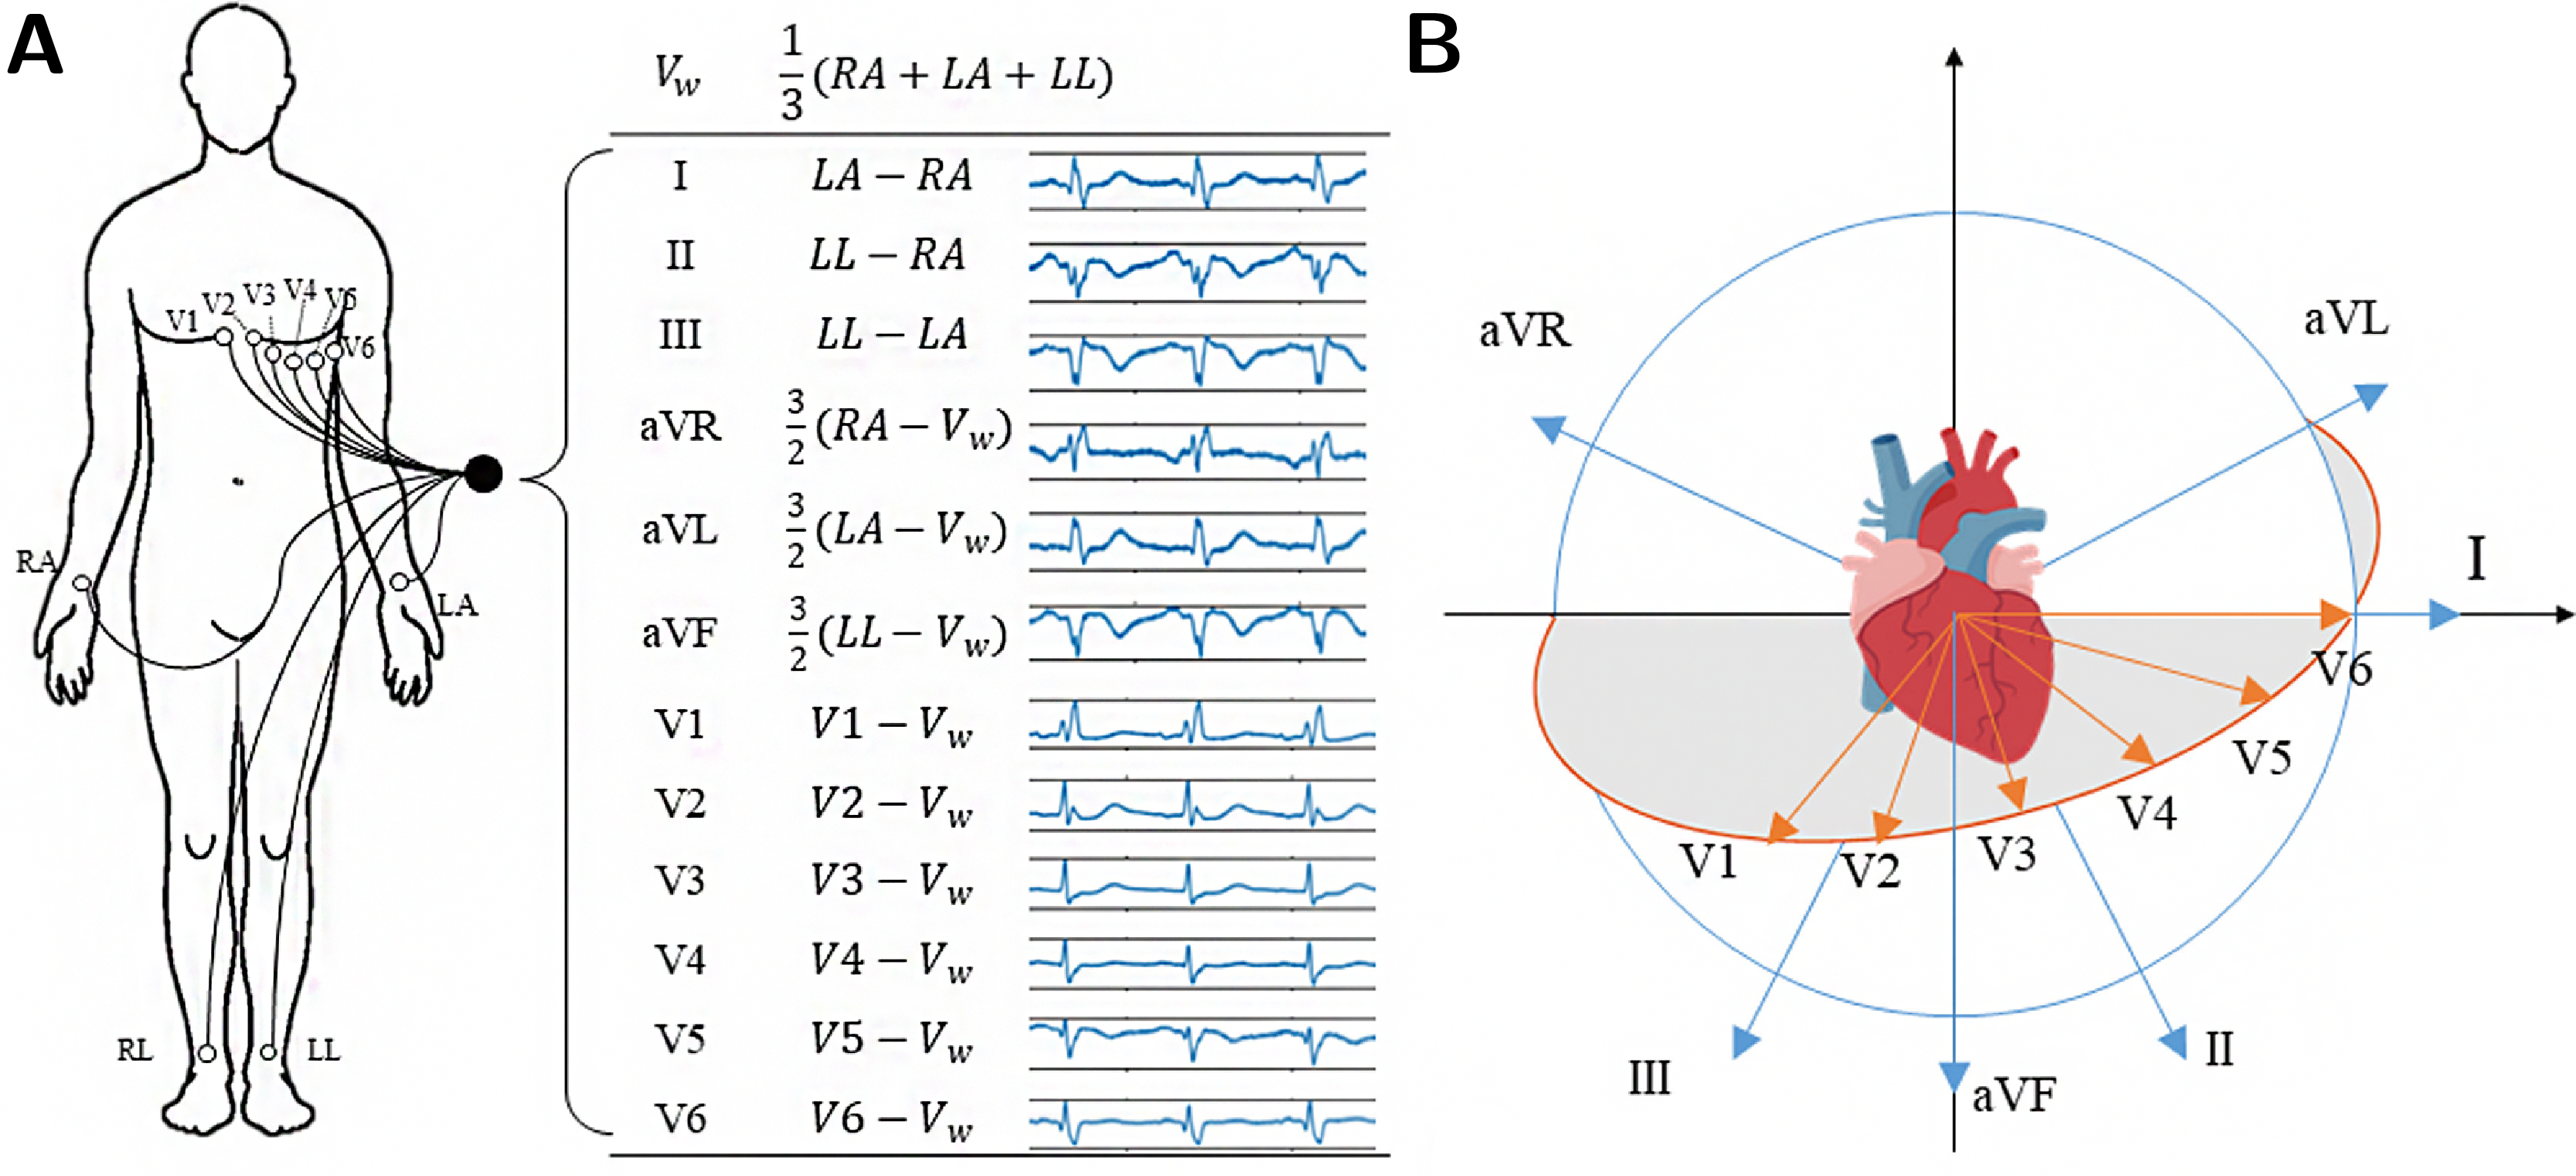
\includegraphics[width=1\linewidth]{figures/ecg_leads}
        \caption{Ilustrace 12svodového EKG systému. \textbf{A)} Prostorové
            rozmístění 10 elektrod: tři končetinové svody, tři rozšířené končetinové
            svody a šest prekordiálních (hrudních) svodů, které byly vytvořeny mezi
            fyzickými elektrodami a virtuální elektrodou známou jako Wilsonův
            centrální terminál ($V_W$). \textbf{B)} Rozdíly elektrických potenciálů
            mezi elektrodami odrážejí elektrickou aktivitu srdce z různých
            prostorových úhlů~(Přeloženo a převzato z~\cite{Yao2020})}
        \label{fig:ecg_leads}
    \end{center}
\end{figure}

\paragraph{Standardní končetinové svody.}
Standardní končetinové svody zachycují rozdíly potenciálů mezi dvěma
končetinami. Elektroda na pravé noze slouží jako referenční, snižuje šum a není
tak součástí konfigurace svodů. Svody jsou uspořádány do trojúhelníku, který se
často nazývá jako Einthovenův trojúhelník. Toto uspořádání zajišťuje, že
potenciál snímaný ve svodu II odpovídá součtu potenciálů měřených ve svodech I a
III~\cite{Goldberger2017,mirvis2001}.

\paragraph{Prekordiální svody a wilsonův centrální terminál.}
Prekordiální svody se používají k záznamu potenciálu v každém ze šesti určených
míst trupu vzhledem k referenci. Na každé místo se umístí aktivní elektroda
připojená ke kladnému vstupu záznamového systému. Referenčním vstupem je složená
elektroda známá jako Wilsonova centrální svorka, která je vytvořena kombinací
výstupu elektrod levé paže (LA), pravé paže (RA) a levé nohy (LL)
prostřednictvím odporů (5000~\si{\ohm})~\cite{Goldberger2017,mirvis2001}.

\paragraph{Rozšířené končetinové svody.}
Jak již bylo zmíněno, třemi augmentovanými svody jsou aVR, aVL a aVF. U svodu
aVR je aktivní elektrodou sloužící jako pozitivní vstup elektroda pravé paže,
zatímco u svodu aVL je to elektroda levé paže a u svodu aVF elektroda levé nohy.
Referenční potenciál je zde vytvořen spojením dvou končetinových elektrod, které
se nepoužívají jako aktivní. Účelem tohoto modifikovaného referenčního systému
je generovat signál s vyšší amplitudou než při použití Wilsonovy centrální
svorky jako referenční elektrody~\cite{Goldberger2017,mirvis2001}.

\paragraph{Další svodové systémy.}
Byly vyvinuty různé svodové systémy, které umožňují detekovat diagnosticky
významné informace, jež nemusí být zachyceny standardním 12svodovým EKG, a
zlepšit efektivitu záznamu, přenosu a ukládání EKG. Používají se například levé
zadní svody k detekci akutních posterolaterálních infarktů nebo elektrodová pole
o 80 nebo více elektrodách k zobrazení potenciálů povrchu těla jako izopotenciálních
map~\cite{Goldberger2017,mirvis2001}. Přehled dalších svodových systému včetně
nositelných byl popsán v~\cite{Baig2013,Majumder2018,Serhani2020}.

\subsubsection{Elektrodermální aktivita}
V úvodu kapitoly bylo řečeno, že princip měření EDA je založen na skutečnosti,
že činnost potních žláz v kůži, která je regulována sympatickým nervovým
systémem, vede ke změnám vodivosti kůže. Díky tomu, a jak může vyplývat z
minulých kapitol, je měření EDA běžně používanou metodou pro hodnocení
fyziologických reakcí souvisejících s emočními a kognitivními procesy.

\begin{figure}[htb!]
    \begin{center}
        \includegraphics[width=1\linewidth]{figures/EDA}
        \caption{\textbf{A)} Možná místa měření kožní vodivosti. \textbf{B)}
            Typická odezva elektrodermální aktivity~(Upraveno a převzato
            z~\cite{Janssen2012,Vavrinsky2021})}
        \label{fig:eda_mereni}
    \end{center}
\end{figure}

Měření elektrodermální aktivity zahrnuje umístění dvou elektrod na kůži, přičemž
jedna měří rozdíly potenciálů mezi dvěma body na kůži a druhá slouží jako
referenční elektroda. Elektrody se obvykle umísťují na prsty nebo dlaň ruky, i
když lze použít i jiná místa, například chodidla nebo čelo (viz
Obr.~\ref{fig:eda_mereni}A) a měří se elektrická vodivost kůže v reakci na malý
stejnosměrný nebo střídavý proud proud~\cite{Caruelle2019,Boucsein2012}.

Z pohledu způsobu měření elektrodermální aktivity lze tedy rozlišovat dvě hlavní
kategorie: endosomatická a exosomatická měření. V rámci endosomatického měření
se zaznamenává pouze potenciál generovaný kůží bez použití vnějšího zdroje. U
exosomatického měření se využívají externí zdroje, jako je právě střídavý nebo
stejnosměrný proud přiváděný na kůži. Aplikace konstantního stejnosměrného
napětí nebo proudu umožňuje měření vodivosti kůže (resp. odporu kůže podle
Ohmova zákona). Pokud se ale aplikuje konstantní střídavé napětí nebo proud, tak
lze měřit kožní admitanci (resp. kožní impedanci). Nejpoužívanější metodou pro
exosomatická měření je metoda stejnosměrného konstantního napětí, a to primárně
díky jednoduššímu procesu vyhodnocování a interpretace než je tomu tak u
endosomatického způsobu~\cite{Boucsein2012,Li2022,Posada2020,Caruelle2019}.

Měřená kožní vodivost nebo kožní potenciál se vyjadřují v jednotkách vodivosti
(mikrosiemens, \si{\micro\siemens}) a napětí (\si{\milli\volt}). V naměřeném
signálu se odrážejí změny v různých časových škálách, které se běžně dělí na dvě
složky: tonickou (\gls{SCL}) a fázickou (\gls{SCR}). Tonická složka představuje
velikost kožní vodivosti nebo potenciálu v nepřítomnosti sudomotorické nervové
aktivity\footnote{Sudomotorická nervová aktivita se vztahuje k \gls{ANS}
    kontrole aktivity potních žláz v reakci na různé environmentální a individuální
    faktory.}, zatímco ta fázická se týká rychlých změn kožní vodivosti nebo
potenciálu jako přímého důsledku sudomotorického vzruchu. Fázická složka je
charakterizován nástupem (SCR ris.), dobou nárůstu (SCR ris. t.), amplitudou
(SCR amp.) a dobou zotavení (SCR rec. tc.). Na Obr.~\ref{fig:eda_mereni} lze
vidět průběh EDA složek společně s jejich korespondujícím popisem. Tonické a
fázické složky lze oddělit pomocí technik zpracování
signálu~\cite{Boucsein2012,Li2022,Posada2020,Caruelle2019,Caruelle2019}.

\subsubsection{Respirační aktivita}
\label{subsec:respiracni_aktivita}
Pro měření dechové aktivity (resp. dechové frekvence) je k dispozici mnoho
metod, od přímého měření ventilace až po nepřímé měření pohybů souvisejících s
dýcháním. V této sekci je stručný přehled často používaných metod měření dechové
aktivity.

\begin{figure}[htb!]
    \begin{center}
        \includegraphics[width=1\linewidth]{figures/rsp_measure}
        \caption{Různé technologie pro měření dechové frekvence ($f_R$). Nahoře
        z kategorie snímačů proudění vzduchu, kde $ΔP(Q)$ je změna úbytku tlaku
        způsobená prouděním vzduchu $Q$. Uprostřed z kategorie snímačů teploty,
        kde $R(T)$ je změna odporu způsobená vlivem teploty $T$. Dole z
        kategorie tenzometrických snímačů, kde $f(\mathcal{E})$ je změna odporu
        způsobená deformačním tlakem $\mathcal{E}$. $V(X)$ je výstupní
        napětí~(Upraveno a převzato z~\cite{Massaroni2019})}
        \label{fig:rsp_mereni}
    \end{center}
\end{figure}

Jednou z nejběžnějších metod měření dechové aktivity je přímé měření ventilace.
Ventilace je celkový objem vzduchu, který se během každého nádechu přesune do
plic a z plic ven, a lze ji měřit pomocí několika technik včetně spirometrie,
pletysmografie, a kapnometrie. Spirometrie měří objem vzduchu, který je
vdechován a vydechován, zatímco pletysmografie měří změny tlaku v uzavřené
komoře během dýchání. Kapnometrie měří koncentraci oxidu uhličitého ve
vydechovaném vzduchu, což úzce souvisí s ventilací. Tyto techniky umožňují
přesné měření dechové aktivity, ale mohou být invazivní a vyžadují
specializované vybavení~\cite{Massaroni2019,Massaroni2021,Liu2019}. 

Alternativní metodou měření dechové aktivity je nepřímé měření pohybů
souvisejících s dýcháním. Tyto pohyby lze detekovat pomocí senzorů umístěných na
hrudníku nebo břiše, jako jsou piezoelektrické senzory, tenzometry nebo
akcelerometry. Tyto snímače detekují změny tvaru nebo pohybu hrudníku nebo
břicha během dýchání a lze je použít k odhadu dechové frekvence a objemu. Tyto
metody jsou méně invazivní než přímé měření ventilace a lze je použít v reálném
prostředí, avšak u některých populací nebo za určitých podmínek mohou být méně
přesné~\cite{Massaroni2019,Massaroni2021,Fazio2021,Liu2019}.

Další nově se objevující metodou měření dechové aktivity je používání
nositelných zařízení, jako jsou chytré hodinky, které mohou detekovat změny
dechových vzorců pomocí fotopletysmografie nebo akcelerometrie.
Fotopletysmografie měří změny objemu krve pomocí světelných senzorů, zatímco
akcelerometrie měří pohyb pomocí pohybových senzorů. Tyto metody jsou
neinvazivní a lze je použít v přirozeném prostředí s tím, že mohou být omezené
ve své přesnosti a preciznosti~\cite{Massaroni2019,Massaroni2021,Fazio2021,
Leube2020,Liu2019,Nam2022,Zschocke2022}. 

\subsection{Postupy zpracování biosignálů}
\label{subsec:postupy_zpracovani_biosignalu}
Zpracování biosignálů označuje techniky a postupy používané k získání informací
z biosignálů, ke zvýšení jejich kvality a k interpretaci jejich významu. V této
sekci je uveden přehled hlavních postupů zpracování biosignálů, včetně jejich
akvizice, předzpracování, extrakce příznaků a klasifikace. 

V návaznosti na předchozí sekci, sběr signálu znamená tedy proces záznamu
biosignálů z lidského těla pomocí měřicích zařízení, jako jsou senzory nebo
elektrody. Kvalita zaznamenaných signálů závisí na různých faktorech, jako je
typ a umístění snímačů, odstup signálu od šumu a vzorkovací frekvence. Například
signály EKG se zaznamenávají pomocí elektrod a jejich umístění ovlivňuje kvalitu
zaznamenaných signálů, protože různé oblasti srdce mohou mít různou sílu nebo
frekvenci signálu. Kromě toho se odstup signálu od šumu týká poměru žádoucího
signálu a nežádoucího šumu v zaznamenaných signálech. Čím vyšší je poměr
signál/šum, tím jsou zaznamenané signály jasnější a spolehlivější. A konečně
vzorkovací frekvence označuje frekvenci, s jakou jsou signály vzorkovány nebo
digitalizovány. Čím vyšší je vzorkovací frekvence, tím přesnější je digitální
reprezentace signálů~\cite{Escabi2005,Karagiannis2011}.

\begin{figure}[htb!]
    \begin{center}
        \includegraphics[width=1\linewidth]{figures/signal_processing_diagram}
        \caption{Řetězec procesů od získání biomedicínského signálu po fázi
        analýzy~(Přeloženo a převzato z~\cite{Karagiannis2011})}
        \label{fig:zpracovani_biosignalu_diagram}
    \end{center}
\end{figure}

Předzpracování se týká postupů používaných k přípravě zaznamenaných signálů pro
další analýzu. Mezi postupy předzpracování patří především filtrování signálu.
Žádoucí je často navržení takového filtru, který rovnou koriguje kolísání nulové
izolinie a potlačuje nežádoucí artefakty (síťový šum, svalové artefakty, apod.).
V některých případech však nestačí pouze frekvenčně selektivní filtrace a volí
se jiné přístupy. Zvolený přístup závisí na zdroji a charakteru signálu.
Porovnání metod předzpracování srdeční, elektrodermální a respirační aktivity
bylo vypracováno v ~\cite{Escabi2005,Khodadad2018,Power2020,Subramanian2019}. 

Extrakce příznaků označuje postupy používané k extrakci relevantních informací
nebo charakteristik z předzpracovaných signálů. Extrakce příznaků je důležitým
krokem při zpracování biosignálů, protože jednak snižuje dimenzionalitu signálů
a také zvýrazňuje právě relevantní informace. Z biosignálů lze extrahovat různé
typy příznaků, například z časové, z frekvenční nebo nelineární
oblasti~\cite{Escabi2005,Karagiannis2011}. Krishnan a Athavale popsali trendy v
extrakci příznaků biomedicínských signálů v~\cite{Krishnan2018}.

Klasifikací se rozumí postupy používané k přiřazení značky (anotace) nebo
kategorie biosignálu na základě jeho extrahovaných vlastností (příznaků).
Klasifikace je dalším důležitým krokem při zpracování biosignálů, protože
umožňuje identifikovat vzory nebo trendy v signálech a předpovídat fyziologický
stav nebo kondici subjektu~\cite{Escabi2005,Karagiannis2011}. Možnosti využití
klasifikace (resp. metod strojového učení) pro biomedicínské aplikace byly
popsány v~\cite{Foster2014,Kording2018,Strzelecki2022}.

Zpracování biosignálů se potýká s různými problémy a omezeními, jako je
variabilita signálů, složitost postupů zpracování a interpretace výsledků.
Variabilitou signálů je myšleno, že biosignály se mohou lišit od subjektu k
subjektu, od sezení k sezení nebo dokonce v rámci jednoho sezení. Tato
variabilita může ovlivnit kvalitu a spolehlivost zaznamenaných signálů a může
vyžadovat použití sofistikovanějších metod předzpracování a
klasifikaci~\cite{Escabi2005,Karagiannis2011}.

\section{Strojové učení}
\label{section:machine_learning}


\subsection{Typy systémů strojového učení}
\subsubsection{Učení s učitelem}
\subsubsection{Učení bez učitele}

\subsection{Trénování a testování modelů}
\subsubsection{Cross-validation} % Křížová validace
\subsubsection{Overfitting and Underfitting} % Přeučení a nedoučení

\subsection{Optimalizace hyperparametrů}

\subsection{Kombinování modelů}

\subsection{Hodnocení modelů}
\subsubsection{Accuracy}
\subsubsection{Predictive Values}
\subsubsection{Area Under the ROC Curve}
\subsubsection{Cross-entropy Loss}
\subsubsection{Bias-varince Tradeoff}

\subsection{Artificial Neural Networks} % Umělé neuronové sítě 
\subsubsection{Single-layer Perceptron} % Jednovrstvý perceptron
\subsubsection{Multi-layer Perceptron} % Vícevrstvý perceptron
\subsubsection{Cost Function}
\subsubsection{Backpropagation and Gradient Descent}
\subsubsection{Optimizers}
\subsubsection{Stochastic Gradient Descent}
\subsubsection{AdaGrad}
\subsubsection{RMSProp}
\subsubsection{Adam}
\subsubsection{Activation Functions}
\subsubsection{Convolutional Neural Networks}
\subsubsection{Convolution}
\subsubsection{Regularization}
\clearpage

\chapter{Cíle práce}
Hlavním cílem diplomové práce je návrh a realizace metod pro hodnocení
kognitivní zátěže z biosignálů současně s vyhodnocením vlivu extrémního
prostředí na její projevy. Hodnocenými biosignály jsou konkrétně elektrická
srdeční aktivita, respirační aktivita a elektrodermální aktivita. Extrémním
prostředím je v kontextu diplomové práce myšlena vesmírná analogová mise.

\clearpage

\chapter{Metody}
\section{Mise DIANA}
\label{sec:mise_diana}
Tato diplomová práce těží z již druhé vesmírné analogové mise, která simulovala
přistání na měsíci a uskutečnila se v rámci projektu Hydronaut v létě roku 2022.
Jednotlivé kompartmenty mise měly následující role: řídící věž byla stanoviště
na Zemi, mateřská loď obíhala na oběžné dráze Měsíce a přistávací modul byl na
povrchu Měsíce. Blíže jsou dílčí kompartmenty popsány v následujících sekcích.

Mise primárně sloužila pro zkoumání vlivu osobnostních charakteristik a vnějších
faktorů na dynamiku týmu při dlouhodobém pobytu v \gls{ICE} prostředí (projekt
TAČR ÉTA č. TL05000228). Mise DIANA byla podpořena Evropskou kosmickou
agenturou, vzhledem k jejímu potenciálu pro výcvik astronautů simulací
extrémního prostředí. 
\subsection{Mise Diana}
\label{subsec:mise_diana}

\subsection{Měření biosignálů}
\label{subsec:_mereni_biosignalu}



\section{Použité datasety}
\label{sec:datasety}
Pro účely diplomové práce bylo použito několik veřejně dostupných datasetů
včetně dat z mise DIANA. V následujících sekcích jsou stručně rozebrány
jednotlivé datasety.
\subsection{WESAD}
\label{subsec:wesad}
Dataset WESAD~\cite{wesadDataset} (\textit{Wearable Stress and Affect
Detection}) je multimodální dataset navržený pro výzkum v oblasti hodnocení
stresu a emocí za použití nositelných senzorů. Tento dataset byl vytvořen s
cílem přispět k vývoji pokročilých algoritmů strojového učení pro analýzu
fyziologických signálů a rozpoznání emocí. WESAD obsahuje data získaná od 15
účastníků, přičemž každý z nich prošel sérií experimentů v laboratorních
podmínkách.

Data byla v datasetu získána ze dvou nositelných zařízení. Prvním zařízením byl
\textit{RespiBAN}\footnote{Zařízení \textit{RespiBAN} již není vyráběno},
nositelný senzor umístěný na hrudi se vzorkovací frekvencí 700~Hz, který
zaznamenával elektrokardiogram, elektrodermální aktivitu, elektromyogram,
respirační signál a teplotu těla. Druhé zařízení byl chytrý náramek
\textit{Empatica E4}\footnote{\url{https://www.empatica.com/research/e4}}, který
zaznamenává krevní tlak (64~Hz), elektrodermální aktivitu (4~Hz), teplotu těla
(4~Hz) a tříosou akceleraci (32~Hz). Experiment, který byl proveden pro sběr
dat, zahrnoval celkem čtyři fáze:
\begin{enumerate}
    \item \textbf{Základní úroveň (Baseline condition)} --- účastník byl požádán, aby
    seděl/stál v klidu po dobu 20 minut.
    \item  \textbf{Stresový úkol (Stress condition)} --- účastník musel pět minut
    přednášet před publikem a poté vyřešit matematický úkol, který byl navržen
    tak, aby vyvolal stres.
    \item  \textbf{Relaxační úkol (Amusement condition)} --- účastník sledoval
    komediální video, které mělo vyvolat příjemné emoce.
    \item  \textbf{Řízená meditace (Meditation)} --- účastník prováděl řízenou
    meditaci, jejíž cílem bylo navození do stavu blízkého neutrálnímu
    afektivnímu stavu.
\end{enumerate}

WESAD poskytuje časově synchronizovaná, předzpracovaná a anotovaná data z těchto
nositelných senzorů. Pro účely diplomové práce byly použity signály ze zařízení
\textit{RespiBAN}, konkrétně srdeční, respirační a elektrodermální aktivita. Pro
úlohy hodnocení kognitivní zátěže byla základní úroveň označena jako klidový stav
a stresové úkoly byly označeny jako stav kognitivní zátěže.

\subsection{CLAS}
\label{subsec:clas}
Dataset CLAS~\cite{clasDataset} (\textit{Cognitive Load, Affect, and Stress
Recognition}) je podobně jako WESAD multimodální dataset vytvořený pro výzkum v
oblasti rozpoznávání kognitivní zátěže a emocí za použití nositelných senzorů a
dalších datových zdrojů. Dataset zahrnuje data získaná od 62 účastníků, kteří
byli vystaveni různým úkolům a podnětům navrženým tak, aby vyvolaly různé úrovně
kognitivní zátěže a emocí. Mezi tyto podněty patřily například matematické úlohy
nebo Stroopův test. Každý účastník byl zároveň měřen i v klidu (dataset stav
označuje jako Baseline). Během přechodů mezi jednotlivými úkoly bylo účastníkům
puštěno neutrální video nebo byl účastník požádán, aby vyplnil dotazník (dataset
označuje jako Neutral). 

Fyziologická data v rámci tohoto datasetu byla měřena zařízením
\textit{Shimmer3}\footnote{\url{https://shimmersensing.com}} se vzorkovací
frekvencí 256~Hz. Mezi měřené biologické signály patří elektrokardiogram,
elektrodermální aktivita a fotopletysmogram. Pro úlohy hodnocení kognitivní
zátěže byl Baseline stav označen jako klidový stav a stresové úkoly byly
označeny jako stav kognitivní zátěže. 

\subsection{Data z vesmírné analogové mise DIANA}
\label{subsec:data_diana}
Pro potřeby diplomové práce poskytla \gls{FF UPOL} data z vesmírné analogové
mise DIANA. Součástí dat jsou osmidenní 24 hodinové záznamy biologických
signálů, kamerových záznamů a anotace v podobě časů kognitivních úloh pro
každého člena posádek. Využitými signály v této práci jsou elektrokardiogram
spolu s elektrodermální a respirační aktivitou.

\section{Zpracování biosignálů}
\label{sec:zpracovani_biosignalu}
Důležitým krokem při analýze biosignálů je jejich zpracování. V této sekci jsou
popsány použité algoritmy, které byly implementovány v programovacím jazyce
Python, využitím knihovny \textit{Neurokit2} (viz sekce~\ref{subsec:neurokit}).
\subsection{Zpracování elektrické srdeční aktivity}
\label{subsec:zpracovani_ekg}
Pro zpracování EKG záznamů byla implementována metoda podle Kalidase a
Tamila~\cite{kalidas2017}, která je založena na stacionární vlnkové transformaci
(\gls{SWT}). Metoda vychází z populárního Pan-Tompkinsova~\cite{Tompkins1985}
algoritmu ale pro odstranění šumu a zvýraznění QRS komplexů používá \gls{SWT}
namísto pásmové propusti. Stacionární vlnková transformace je metoda rozkladu
signálu na jednotlivá frekvenční pásma pomocí mateřské vlnky~\cite{Nason1995}.
Metoda byla zvolena na základě následující sekce~\ref{subsubsec:vyberqrs}.

\begin{figure}[H]
    \begin{center}
        \includegraphics[width=1\linewidth]{figures/kalidas2017}
        \caption{\textbf{A-D)} Kroky zpracování EKG pro algoritmus podle
            Kalidase a Tamila~\cite{kalidas2017} \textbf{E)} Frekvenční spektrum
            nefiltrovaného EKG se vzorkovací frekvencí 250~\si\Hz~(modrá) a EKG po
            SWT 3. řádu (oranžová). \textbf{F)} vlnka rodiny Daubechies 3. řádu.
            (Upraveno a převzato z~\cite{Porr2019})}
        \label{fig:kalidas_processing}
    \end{center}
\end{figure}

V tomto algoritmu se stacionární vlnková transformace provádí na EKG signálu
využitím Daubechiesové vlnky třetího řádu. Po provedení \gls{SWT} se extrahují
koeficienty, které se následně vyčíslí na čtverec. Následně je využito filtrace
pásmovou propustí ke zvýšení citlivosti a přesnosti detekce. Postup detekce R
vln na filtrovaném signálu je pak totožná s detekcí Pan-Tompkinsova
algoritmu~\cite{Tompkins1985}. Jednotlivé částí zpracování lze vidět na
Obr.~\ref{fig:kalidas_processing}.

\subsubsection{Metodika výběru QRS detektoru}
\label{subsubsec:vyberqrs}
Vzhledem k tomu, že neexistuje žádný jednotný standard či systematický postup
pro zpracování EKG a výběr \enquote{správného} QRS detektoru pro určitou
aplikaci, tak bylo v rámci této práce realizováno statistické porovnání
populárních algoritmů. Jakožto měřítko přesnosti QRS detekce algoritmu bylo
vycházeno z výpočtu absolutní vzdálenosti od původní \enquote{skutečné} polohy R
vlny. Pro benchmarking detektorů byly tedy použity následující anotované
datasety:

\begin{table}[h]
    % \footnotesize
    \begin{center}
        \caption{\label{tab:bench_datasets} Vybrané datasety pro benchmarking
            QRS detektorů z PhysioNetu~\cite{PhysioNet}}
        \renewcommand{\arraystretch}{1.3}
        \begin{tabular}{p{12cm}c}
            \toprule
            \textbf{Dataset}                                                                                                 & \textbf{Probandi} \\ \midrule
            MIT-BIH Arrhythmia Database~\cite{MITBIHArrhythmia}                                                              & 48                \\
            MIT-BIH Normal Sinus Rhythm Database~\cite{Beth1990}                                                             & 18                \\
            Glasgow University Database~\cite{GUDB}                                                                          & 25                \\
            Fantasia Database~\cite{FANTASIA}                                                                                & 40                \\
            Lobachevsky University Electrocardiography Database~\cite{LUDB}                                                  & 200               \\
            Simultaneous physiological measurements with five devices at different cognitive and physical loads~\cite{IFADO} & 13                \\
            Pulse Transit Time PPG Dataset~\cite{USYD}                                                                       & 22                \\
            \bottomrule
        \end{tabular}
    \end{center}
\end{table}

Byly vybrány různorodé datasety za účelem zjištění adaptability algoritmu. Pro
statistické zpracování bylo využito lineárních smíšených modelů (\gls{LMM}).
Použité statistické metody jsou podrobněji popsány v
kapitole~\ref{sec:statisticke_metody}. Pro srovnání metod byl v programovacím
jazyce R vytvořen následující statistický model:
\begin{equation}
    \text{Skóre} = \beta_0 + \beta_1\text{Metoda} + u_{\text{Dataset}} + u_{\text{Participant}} + \epsilon
\end{equation}
který specifikuje lineární smíšený model pomocí funkce \texttt{lmer} z balíku
\texttt{lme4}\footnote{\url{https://github.com/lme4/lme4}}. Model byl použit k
predikci závislé proměnné Skóre na fixním efektu $Metoda$ a dvou náhodných
efektech: $Dataset$ a $Participant$. Dále problematice této sekce není věnována
pozornost, jelikož není předmětem této práce. 

\subsection{Zpracování respirační aktivity}
\label{subsec:zpracovani_rsp}
Pro zpracování respirační aktivity byl implementován
algoritmus~\cite{Khodadad2018}, který je založen na průchodech nulou (\gls{ZC},
Zero-Crossing). Originální signál je nejdříve filtrován pásmovou propustí pro
odstranění stejnosměrné složky, aby bylo možné spolehlivě detekovat \gls{ZC}. K
tomu byla využita pásmová propust 0,05--3~Hz , která zároveň zachovává dechové
frekvence menší než tři a vyšší než 180 dechů za minutu. Následně jsou pomocí
logických operací detekovány indexy náběžných a sestupných průchodů nulou, mezi
kterými došlo k hledání lokálních extrémů.

\begin{figure}[h]
    \begin{center}
        \includegraphics[width=1\linewidth]{figures/rsp_test}
        \caption{Příklad zpracování RSP pomocí implementované metody}
        \label{fig:rsp_test}
    \end{center}
\end{figure}

Zachovány jsou ve výsledku pouze ty extrémy, které mají minimální vertikální
vzdálenost od svého přímého souseda, tudíž kritérium pro detekci odlehlých
hodnot bylo definováno v absolutním rozdílu amplitud mezi sousedními extrémy.
Aplikace metody na reálném signálu lze vidět na Obrázku~\ref{fig:rsp_test}.

\subsection{Zpracování elektrodermální aktivity}
\label{subsec:zpracovani_eda}
Zpracování elektrodermální aktivity vychází z metod~\cite{vanhalem2020}
a~\cite{posada2016}. Signál je nejdříve filtrován Butterworthovou horní propustí
4. řádu s mezní frekvencí 3~\si\Hz. Následně je ze signálu extrahována fázická a
tonická složka pomocí dolní a horní propusti o mezních frekvencích 0,05~\si\Hz.

\begin{figure}[h]
    \begin{center}
        \includegraphics[width=1\linewidth]{figures/eda_test}
        \caption{Příklad zpracování EDA pomocí implementovaných metod}
        \label{fig:eda_test}
    \end{center}
\end{figure}

Dále byl použit Savitzky-Golayův frekvenčně neselektivní filtr k dalšímu
vyhlazení fázické složky za účelem hledání \gls{SCR} vrcholků. K detekti
vrcholků byla využita funkce \texttt{find\_peaks()} z knihovny
Scipy\footnote{\url{https://docs.scipy.org}}. Kritérium pro detekci vrcholků
bylo definováno jako konzistentní nárůst o 0,5s následovaný stejným poklesem.
Výsledek aplikované metody lze vidět na Obrázku~\ref{fig:eda_test}.

\subsection*{Neurokit}
\label{subsec:neurokit}
Knihovna \textit{Neurokit2}\footnote{\url{https://neuropsychology.github.io/NeuroKit}},
na jejíž vývoji se podílím, poskytuje pokročilé metody pro zpracování a
vizualizaci biosignálu. Jednotlivé metody zároveň nabízejí možnost si vybrat z
mnoha implementovaných algoritmů. V této práci byla knihovna použita pro
zpracování respirační, elektrodermální a elektrické srdeční aktivity včetně
zpracování a výpočet \gls{HRV} parametrů.


\section{Zpracování dat z mise DIANA}
\label{sec:zpracovani_dat_diana}
\subsection{Zpracování exportovaných segmentů biosignálů}
\label{subsec:prezpracovani_segmentu}
Pro každého člena posádky byly exportovány segmenty biosignálů o délce 30s s
50\% překryvem na základě poznatků
v~\cite{Castaldo2019,Kim2021,Pecchia2018,Shaffer2020,Tervonen2021}. Zpracování
biosignálu vycházelo z metodiky popsané v sekci~\ref{sec:zpracovani_biosignalu}.
U každého segmentu proběhlo hodnocení jeho kvality podle dvou kritérií:
\begin{itemize}
    \item Hodnocení kvality \gls{EKG} signálu pomocí heuristické fúze a fuzzy
    komplexního hodnocení podle~\cite{Zhao2018}.
    \item Hodnocení detekovaných R vln z hlediska časové kontroly náhlých
    nefyziologických změn v po sobě jdoucích R-R intervalech.
\end{itemize}
Segmenty které vykazovali nežádoucí anomálie v rámci hodnotících kritérií byly
vyřazeny. Ze segmentů bylo dále vypočteno následně přes 100 různých parametrů
pro účely analýzy dat. Mezi tyto parametry patřily například běžné statistické
charakteristiky (průměr, medián, směrodatná odchylka a další) nebo nelineární a
časové \gls{HRV} parametry. Zpracované segmenty byly zároveň anotovány, a to z
hlediska spánkového cyklu. Dále byly identifikovány a označeny v časech
kognitivních testů. Z časových důvodu nebyly pro účely této práce ostatní
aktivity během mise anotovány, i přes dostupnost kamerových záznamů. Seznam
všech počítaných parametrů je součástí přílohy v souboru
\texttt{all\_params.csv}.

\subsection{Čistění dat}
\label{subsec:cisteni_dat}
Ze souborů vypočtených parametrů byly vynechány všechny parametry, jejichž
sloupce obsahovali \texttt{NaN} hodnoty. Dále byly parametry korelovány a
odstranili se ty, které byly vzájemně dokonale korelované ($|r| > 0,999$). Poté
se odstranili odlehlé hodnoty na základě absolutní odchylky mediánu od mediánu.

\subsection{Sledované veličiny}
\label{subsec:sledovane_veliciny}
Pro účely analýzy \gls{NPF} adaptace probandů v průběhu mise byly vybrány a
sledovány především následující \gls{HRV} parametry:

\subsection{Tvorba hypotetických LMM modelů}
\label{subsec:tvorba_modelů}



\section{Explorační analýza dat}
\label{sec:exploracni_analyza}
\subsection{Předzpracování datasetů}
\label{subsec:predzpracovani_datasetu}
Z datasetů byly extrahovány potřebné biosignály, které byly následně zpracovány
a normalizovány na úrovní subjektů. Metodika zpracování vychází ze
sekce~\ref{sec:zpracovani_biosignalu}. Normalizace byla provedena škálováním
biosignálů tak, aby měly průměrnou hodnotu nula a směrodatnou odchylku jedna. To
bylo dosaženo odečtením střední hodnoty biosignálu od každé jeho hodnoty a
následným vydělením směrodatnou odchylkou.

Vzhledem k tomu, že dataset CLAS neobsahuje signál RSP, byl tento signál
vytvořen pomocí metody \gls{EDR} (ECG-Derived Respiration). Jedná se o extrakci
informace o dýchání z elektrokardiogramu. Knihovna \textit{Neurokit2} poskytuje
implementaci algoritmu podle~\cite{VanGent2019}, jež byla pro tyto účely
použita.

Následně byly všechny signály segmentovány na 5s, 5s s 50\% překryvem a 1s
úseky. Z těchto segmentů byly poté vytvořeny příznaky pro účely strojového
učení. Blíže je tvorba těchto příznaků a jejich využití popsáno v
sekci~\ref{sec:hybridni_detekce}. Byly ponechány pouze ty segmenty, které svojí
třídou korespondovaly žádanému kognitivnímu stavu.

\begin{figure}[h]
    \centering
    \framebox[\textwidth]{%
        \begin{subfigure}[b]{0.45\textwidth}
            \dirtree{%
                .1 Datasets.
                .2 WESAD.
                .3 S2.
                .4 S2.pkl.
                .4 $\vdots$.
                .3 S3.
                .3 $\vdots$.
                .2 CLAS.
                .3 Part1.
                .4 full\_ecg.csv.
                .4 full\_gsr\_ppg.csv.
                .4 $\vdots$.
                .3 Part2.
                .3 $\vdots$.
            }
            \caption{Původní struktura datasetů}
            \label{subfig:tree1}
        \end{subfigure}
        \hfill
        \begin{subfigure}[b]{0.45\textwidth}
            \dirtree{%
                .1 Datasets.
                .2 WESAD.
                .3 merged\_1s.pkl.
                .3 merged\_5s.pkl.
                .3 merged\_5s\_2s.pkl.
                .3 $\vdots$.
                .2 CLAS.
                .3 merged\_1s.pkl.
                .3 merged\_5s.pkl.
                .3 merged\_5s\_2s.pkl.
                .3 $\vdots$.
            }
            \caption{Zpracované datasety}
            \label{subfig:tree2}
        \end{subfigure}
    }
    \caption{Porovnání struktury původních a zpracovaných datasetů}
    \label{fig:struktura_datasetu}
\end{figure}

\subsection{Explorace dat}
\label{subsec:explorace_dat}
Oba datasety byly po předzpracování zkoumány pomocí nástrojů knihovny
\textit{Pandas} v programovacích jazyce Python. Datasety tak byly popsány
například základními statistickými údaji, kde byla brána primárně zřetel na
rozdělení tříd. Na Obr.~\ref{fig:rozdeleni_trid} lze tak vidět, že oba datasety
vykazují výraznou nevyváženost tříd. Dále byly korelovány jednotlivé signály
datasetů, bylo nahlíženo na jejich distribuce, a byly vyšetřeny případné záporné
nebo neplatné hodnot. Tato šetření byla provedena i na individuální úrovni. Celý
postup s vizualizovanými výsledky se nachází v datové příloze, v podobě
interaktivního prostředí Jupyter Notebook\footnote{\url{https://jupyter.org}} s
názvem souboru \texttt{exploratory\_analysis\_example}.

\begin{figure}[h]
    \begin{subfigure}[h]{0.48\linewidth}
        \includegraphics[width=\linewidth]{figures/wesad_labels}
        \caption{Rozdělení datasetu WESAD}
    \end{subfigure}
    \hfill
    \begin{subfigure}[h]{0.48\linewidth}
        \includegraphics[width=\linewidth]{figures/clas_labels}
        \caption{Rozdělení datasetu CLAS}
    \end{subfigure}
    \caption{Srovnání rozdělení tříd vybraných datasetů. Třída 0 vyjadřuje
    klidový stav a třída 1 vyjadřuje kognitivní zátěž.}
    \label{fig:rozdeleni_trid}
\end{figure}

Během explorace dat byla také zkoumána separovatelnost dat v
nízkodimenzionálních prostorech použitím techniky \gls{UMAP}~\cite{umap2018}
(Uniform Manifold Approximation and Projection) právě pro redukci
dimenzionality. Cílem bylo vizualizovat soubor dat ve formě nižších dimenzí k
získání přehledu o rozdělení tříd a nadhled nad smyslem a rozpoložení dat.
Výsledky této vizualizace je možné vidět na Obr.~\ref{fig:umap}, kde jsou
oranžově vyznačeny body, jež odpovídají kognitivní zátěži.

\begin{figure}[h]
    \begin{subfigure}[h]{0.48\linewidth}
        \includegraphics[width=\linewidth]{figures/wesad_umap}
        \caption{WESAD}
    \end{subfigure}
    \hfill
    \begin{subfigure}[h]{0.48\linewidth}
        \includegraphics[width=\linewidth]{figures/clas_umap}
        \caption{CLAS}
    \end{subfigure}
    \caption{Vizualizace UMAP projekcí extrahovaných příznaků z datasetu WESAD
    do 2D (vlevo) a 3D latentního prostoru (vpravo). Oranžově třída 1 a modře
    třída 0}
    \label{fig:umap}
\end{figure}

V metodě bylo využito Euklidovské vzdálenostní metriky s hodnotou 0,1 a počtem
sousedních bodů 15. Tyto nízké hodnoty byly zvoleny pro účely zachycení lokální
struktury dat (potenciálně na úkor celkového obrazu), jak ukazuje
Obr.~\ref{fig:umap}. Výsledek 3D projekcí naznačuje potencionální lineární
separovatelnost u malé části souboru. U zbytku souboru by bylo oddělení
pravděpodobně zřetelnější ve vyšších dimenzích a možná nebude lineární. V úvahu
tak přichází strojové učení.

\section{Konvenční parametrická detekce CL}
\label{sec:kovencni_detekce}
\input{chapters/metody/konvencni_detekce}

\section{Detekce CL využitím vícerozměrných časoprostorových kauzálních vzorů}
\label{sec:hybridni_detekce}
\subsection{Definice problému}
\label{subsec:definice_problemu}
V předešlé sekci byl popsán proces předzpracování dat, jehož výsledkem je nová
multidimenzionální množina segmentovaných fyziologických signálů $\mathcal{F}$.
Dimenze této množiny je rovna počtu snímaných signálů, lze tedy dál hovořit jako
o kanálech $c$. Vybraný segment z kanálu $c$ reprezentuje časovou řadu, jejiž
každý vzorek je zachycen v určitém čase $t$, a představuje průběh fyziologické
události (\gls{NPF} událost).

Mezi jednotlivými pozorovanými fyziologickými událostmi $X^i$, lze modelovat
časově kauzální vztahy, které lze díky Grangerově kauzalitě (viz
sekce~\ref{subsec:granger}) matematicky popsat unikátním orientovaným grafem --
definovanou množinou vrcholů a hran. Tím je umožněno temporální kódování
specifického příčinného kognitivního stavu pro konkrétní segment vybraného
kanálu $c$. Nelze však předpokládat, že je tak zachycena veškerá komplexní
dynamika, která je ve biosignálech přítomna, včetně toho, že nemusí být plně
zachyceny interakce napříč kanály $c$.

Tento problém je kompenzován použitím vícerozměrných časoprostorových vzorů
(\gls{GAF}, Gramian Angular Fields) odvozených z Gramových matic. Tyto vzory
zachycují určitý druh temporální i prostorové korelace v rámci fyziologických
událostí. V následujících sekcích je dále popsána tvorba zmíněných příznaků
společně s jejich aplikací v rámci strojového učení.

\subsection{Tvorba kauzálních vícerozměrných matic}
\label{subsec:kauzalni_matice}
Pro zachycení časově kauzálních relací v použitých biosignálech byl zvolen
přístup Kopula-Granger s Lasso ($\ell_1$) regularizací, který kombinuje koncept
Grangerovy kauzality s teorií kopulí. Zmíněné přístupy spadají do oblasti
statistických metod, a proto jsou dále jednotlivé popsány v
sekci~\ref{sec:statisticke_metody}.

Vytvoření kauzální matice ja založeno na použití fyziologické události $X^i$
definované v minulé sekci, ze které lze uplatněním Kopula-Granger metody získat
robustní odhad koeficientů vektorů $\beta_i$ pro test Grangerovy kauzality
využitím regresní úlohy. K tomu je ale potřeba vyřešit následující optimalizační
problém~\cite{Schindler2013,Guy2016}:
\begin{equation}
    \min _{\beta_i} \sum_{l=L+1}^T\left|X_t^i-\sum_{j=1}^p\left(X_{t, \text {lag}}^j\right) \cdot\left(\beta_i^j\right)^{\prime}\right|^2+\lambda\left\|\beta_i\right\|_1,
\end{equation}
kde $\lambda$ je penalizační parametr ovlivňující řídkost vektoru $\beta_i$, $L$
je maximální časové zpoždění (lag) a ${X}_{t, \text {lag}}^j$ jsou předchozí
hodnoty řady $X^j$ v čase $[t - L, t - 1]$. Podle definice Kopula-Granger
modelu~\cite{Schindler2013,Guy2016} lze dále uplatnit faktorizaci na základě
modelu vektorové autoregrese (\gls{VAR}) s koeficienty $B = {{\beta}_{i}^j}$
následovně:
\begin{equation}
    p_Z(z)=\mathcal{N}(z(1, \ldots, L)) \times \prod_{j=1}^n \prod_{t=L+1}^T p_{\mathcal{N}}\left(z_j(t) ; \sum_{t=1}^n \beta_{i, j}^T z_i^{t, \text {lag}}, \sigma_j\right)
\end{equation}
kde $p_{\mathcal{N}}(z ; \mu, \sigma)$ je Gaussova funkce se střední hodnotou
$\mu$ a rozptylem $\sigma^2$, $z_i^{t, \text {lag}}$ jsou předchozí hodnoty
$z_i$ do času $t$ a ${\beta}_{i}^j$ je vektor koeficientů modelujících vliv
časové řady $z_j$ na cílovou časovou řadu. Kauzalita je tedy definována časovou
řadou $z_j$, jež je příčinou $z_i$ pokud je alespoň jedna hodnota vektoru
${\beta}_{i}^j$ nenulová ve smyslu statistické významnosti
(viz~\ref{subsec:granger}).

\begin{figure}[h]
    \begin{center}
        \includegraphics[width=1\linewidth]{figures/GCN}
        \caption{Diagram tvorby kauzálních vícerozměrných matic. 1) Aplikace
            Kopula-Granger metody pro vybraný segment všech kanálů $c$. 2) Kombinace
            výsledných kauzálních matic do jednoho trojrozměrného pole. 3) Výsledný
            příznak ve smyslu RGB obrázku}
        \label{fig:GCN}
    \end{center}
\end{figure}

Kopula-Granger metodu lze primárně shrnout do dvou kroků: odhadnutí marginální
distribuční funkce vybrané časové řady $X^i$ jako $\hat{F_i}$ a mapování
pozorovaných hodnot fyziologické události v čase $t$ do kopula prostoru jako
$Z_{i}^t=\Phi^{-1}\left(\hat{F}_i\left(X_{t}^i\right)\right)$, kde $\Phi$ je
kumulativní distribuční funkce (\gls{CDF}) Gaussova rozdělení. V neposlední řadě
lze konstruovat temporální kauzální graf analýzou relací mezi $Z_{i}^t$. Pro
účely tvorby grafického řešení v podobě kauzální matice $T \times T$ obsahující
odhady koeficientů $\hat{\beta}_i$ byla adaptována regularizovaná regrese
podle~\cite{Bahdori2012}:
\begin{equation}
    \hat{\beta}_i(\lambda)=\arg \min _{\beta_i}\left(\sum_{t=1}^T\left\|x_i^t-X_{t, L}^{\text {lag}} \beta_i\right\|^2+\lambda\left\|\beta_i\right\|_1\right)
\end{equation}
kde $x_i^t$ představuje pozorovanou hodnotu v časové řadě a $X_{t, L}^{\text {lag}}$
reprezentuje spojený vektor všech zpožděných pozorování. Tvorba
kauzálních matic byla realizována v programovém prostředí Matlab s využitím
knihovny \textit{GLMNET}\footnote{\url{https://hastie.su.domains/glmnet_matlab}},
která umožňuje specifikovat různé typy regresních modelů. Hodnota časového
zpoždění byla určena na základě Akaikeho informačního kritéria (\gls{AIC}) jako
$L = 4$. Během každého výpočtu bylo pomocí zmíněné knihovny realizováno i
automatické ladění hodnot penalizačního parametru $\lambda \in m_i$, kde $m_i =
    10^{a + (i-1)d}$ pro $i = {1, 2, ..., 6}$ a $d = \frac{b-a}{n-1}$. Hodnoty $a$ a
$b$ byly nastaveny na -3 a 2.

\subsection{Konstrukce časoprostorových polí}
\label{subsec:gadf}
Bylo realizováno mapování segmentů všech kanálů $c$ do prostorové domény
(\gls{GAF}), jež zachovává časové závislosti. Wang and Oates~\cite{Wang2015}
představili koncept této metody transformace časové řady do 2D obrazu v roce
2015. Vzhledem k dříve definované fyziologické události, tedy vybrané časové
řadě $X^i = \{x_1^i, x_2^i, \dots, x_t^i\}$ z kanálu $c$ zahrnuje konstrukce
\gls{GAF} nejdříve normalizaci na interval $[-1; 1]$:
\begin{equation}
    \tilde{x}_t=\frac{\left(x_t-\max (X^i)+\left(x_t-\min (X^i)\right)\right.}{\max (X^i)-\min (X^i)}
\end{equation}

\begin{figure}[h]
    \begin{center}
        \includegraphics[width=1\linewidth]{figures/polar}
        \caption{Ukázka \gls{GAF} mapování na EKG segmentu~(Upraveno a převzato z~\cite{Zhou2021})}
        \label{fig:polar}
    \end{center}
\end{figure}

Dále jsou normalizovaná data časové řady převedeny do polárních souřadnic
výpočtem úhlové složky $\theta_i$ a radiální složky $r_i$ pro každý vzorek
$\tilde{x}_t$:
\begin{equation}
    \begin{cases}
        \theta_i = \arccos(\tilde{x}_t), & -1 \leq \tilde{x}_t \leq 1, \tilde{x}_t \in \tilde{X^i} \\
        r_i = \frac{t}{N},               & t \in N
    \end{cases}
\end{equation}
kde $t$ je časová značka vzorku fyziologické události a $N$ je konstantní faktor
pro regulaci rozpětí polárního souřadného systému. Jinými slovy, časová značka
představuje poloměr a arkus kosinus hodnoty časové řady úhel. Lze zde hovořit o
bijektivní transformaci, jež zachovává časovou závislost pomocí souřadnice $r$.

Po transformaci přeškálované časové řady do polárního souřadnicového systému lze
využít úhlovou perspektivu, v tomto případě s ohledem na trigonometrický rozdíl
mezi jednotlivými body (\gls{GADF}, Gramian angular field difference), k
identifikaci temporální korelace v rámci různých časových intervalů:
\begin{equation}
    GADF = \left[\sin \left(\phi_i-\phi_j\right)\right]
\end{equation}

\begin{figure}[h]
    \begin{center}
        \includegraphics[width=1\linewidth]{figures/GADF}
        \caption{Diagram tvorby časoprostorových vzorů. 1) Aplikace GAF mapování
            pro vybraný segment všech kanálů $c$. 2) Kombinace výsledných polí
            do jednoho trojrozměrného pole. 3) Výsledný příznak kódující
            temporální korelace fyziologické události v prostorové doméně}
        \label{fig:gadf}
    \end{center}
\end{figure}

Ve výsledku je tedy časoprostorový vzor definován následující $T \times T$
maticí, která je kvazi-Gramovou maticí:
\begin{equation}
    GADF = \left[\begin{array}{cccc}
            \sin \left(\phi_1-\phi_1\right) & \sin \left(\phi_1-\phi_2\right) & \cdots & \sin \left(\phi_1-\phi_n\right) \\
            \sin \left(\phi_2-\phi_1\right) & \sin \left(\phi_2-\phi_2\right) & \cdots & \sin \left(\phi_2-\phi_n\right) \\
            \vdots                          & \vdots                          & \ddots & \vdots                          \\
            \sin \left(\phi_n-\phi_1\right) & \sin \left(\phi_n-\phi_2\right) & \cdots & \sin \left(\phi_n-\phi_n\right)
        \end{array}\right]
\end{equation}
kde každý prvek odpovídá sinové funkci úhlového sinusového rozdílu v různých
časových bodech. Výpočet a tvorba těchto příznaků, časoprostorových vzorů, byla
implementována v programovacím jazyce Python.

\subsection{Augmentace dat}
\label{subsec:augmentace_dat}

\subsection{Kapsulární neuronová síť}
\label{subsec:kapsularni_sit}
Pro potřeby realizace úloh klasifikace (resp. detekce kognitivní zátěže), byla
navržena architektura kapsulární neuronové sítě postavená na řešení, které
představili Mazzia et al.~\cite{Mazzia2021}, \textit{Efficient-CapsNet}.
Celkovou architekturu lze vidět na obrázku~\ref{fig:architektura}.

\begin{figure}[h]
    \begin{center}
        \includegraphics[width=1\linewidth]{figures/capsule}
        \caption{Schematické znázornění architektury sítě
            \textit{Efficient-CapsNet} (Upraveno a převzato z~\cite{Zhou2021})}
        \label{fig:architektura}
    \end{center}
\end{figure}

Zjednodušeně, v případě použití jednoho příznaku, je vstupem modelu obraz, který
lze reprezentovat jako tenzor $X$ s tvarem $H \times W \times C$, kde $H$, $W$ a
$C$ jsou výška, šířka a kanály. V našem případě se jedná o synergické spojení
dvou sad příznaků vyplývajících z minulých sekcí, kauzálních matic $X_{COG} \in
    \mathbb{R}^{T \times T \times C}$ a časoprostorových vzorů $X_{GAF} \in
    \mathbb{R}^{T \times T \times C}$. Vstupním tenzorem je tedy příznak $X \in
    \mathbb{R}^{2 \times T \times T \times C}$. Než se vstup dostane k primární
kapsulové vrstvě, tak je provedena extrakce lokálních vlastnosti ze vstupu $X$
pomocí sady několika typů vrstev\footnote{Jednotlivé vrstvy jsou pojmenovány
    podle korespondujícího názvu v \textit{TensorFlow} a \textit{Keras} API}:
\begin{itemize}
    \item \textbf{Conv2D} --- Tato vrstva vytváří konvoluční jádro, které je
          konvolvováno se vstupem vrstvy a vytváří tenzor výstupů. V podstatě se jedná
          o sadu naučitelných filtrů. Každý filtr transformuje část obrazu
          (definovanou velikostí jádra) pomocí filtru jádra. Matice jádrového filtru
          se aplikuje na celý obraz. Filtry lze chápat jako transformaci obrazu.
    \item \textbf{BatchNormalization} --- Tato vrstva aplikuje normalizaci,
          která udržuje průměrný výstup blízko nule a směrodatnou odchylku výstupu
          blízko jedné.
    \item \textbf{MaxPool2D} --- Tato vrstva funguje jednoduše jako filtr pro
          podvzorkování. Podívá se na 2 sousední pixely a vybere maximální hodnotu.
          Slouží ke snížení výpočetní náročnosti a do jisté míry také ke snížení
          přeučení.
    \item \textbf{Dropout} --- Dropout je regularizační metoda, při níž je část
          uzlů ve vrstvě náhodně ignorována (nastaveny na nulu) pro každý
          tréninkový vzorek. Tím se náhodně vynechá část sítě a síť je nucena
          učit se funkce distribuovaným způsobem. Tato technika také zlepšuje
          generalizaci a snižuje přeučení.
\end{itemize}

\begin{figure}[h]
    \begin{center}
        \includegraphics[width=0.85\linewidth]{figures/conv}
        \caption{První část sítě ($H_{Conv}$), která mapuje vstupní obraz na
            prostor vyšší dimenze}
        \label{fig:conv}
    \end{center}
\end{figure}

Každý výstup konvoluční vrstvy $l$ se tedy skládá z konvoluční operace s určitou
rozměrovou velikostí kernelů $k$ a počtem příznakových map $f$. U konvolučních
vrstev byla použita aktivační funkce $\operatorname{ReLU}$ k přidání nelinearity
do sítě:
\begin{equation}
    F^{l+1}\left(X^l\right)=\operatorname{ReLU}\left(\text {Conv}_{k \times k}\left(X^l\right)\right)
\end{equation}
Celkově si lze první část sítě představit jako jednu funkci $H_{Conv}$, která
mapuje vstupní obraz do prostoru s vyšší dimenzí, což usnadňuje tvorbu
kapslí\footnote{\enquote{Kapsle} označuje skupinu neuronů, která společně
představuje instanci parametru specifické entity nebo části obrazu}. Tuto první
část sítě lze vidět na Obr.~\ref{fig:conv}. Následně je pak využito hloubkově
oddělitelné konvoluce, ze které je získána vrstva primárních kapslí $S_{n,d}^l$
kde $n^l$ a $d^l$ jsou počty primárních kapslí a jejich jednotlivé rozměry
$l$-té vrstvy. Základním prvkem sítě tedy již není jeden neuron, ale vektorová
výstupní kapsle, která by měla zachovávat svojí orientaci a délku. To je
realizováno pomocí \enquote{\textit{squash}} aktivační funkce:
\begin{equation}
    \operatorname{squash}\left(s_n^l\right)=\left(1-\frac{1}{e^{\left\|s_n^l\right\|}}\right) \frac{s_n^l}{\left\|s_n^l\right\|}
\end{equation}
kde $s_n^l$ označuje právě jednu kapsli. Detailně koncept kapsulární sítě popsal
Hinton~\cite{Hinton2011}. Kapsulární neuronová síť byla implementována v
programovacím jazyce Python využitím knihoven
\textit{TensorFlow}\footnote{\url{https://www.tensorflow.org}} a
\textit{Keras}\footnote{\url{https://keras.io}}. Počet filtrů konvolučních
vrstev byl zvolen 32, 64, 64 a 128 v pořadí, tak jak jdou za sebou ve
schématu~\ref{fig:conv}. Velikosti kernelů byly zvoleny 5, 3, 3 a 3. MaxPool2D
vrstvy byly přidány k zajištění kombinace lokálních rysů příznaků a učení se tak
jeho globálnějším rysům. 

\subsection{Self-attention směrování}
\label{subsec:dynamicke_smerovani}

\subsection{Marginální ztrátová funkce}
\label{subsec:marginalni_funkce}
V případě této práce se jedná o binární a vícetřídový klasifikační problém, pro
který by se za normálních okolností použila ztrátová funkce ve smyslu binární
nebo kategorické křížové entropie. Tyto ztrátové funkce ale nezachycují
sémantiku vektorů, jak je používána v kapslích. Pro tyto potřeby byla využita
marginální ztrátová funkce, kde v případě klasifikace více tříd, je pro každou
třídu reprezentovanou kapslí $n^L$ v poslední vrstvě $L$ vypočtena
pravděpodobnost existence určité třídy následovně:
\begin{equation}
    \mathcal{L}_{n^L}=T_{n^L} \max \left(0, m^{+}-\left\|u_n^L\right\|\right)^2+\lambda\left(1-T_{n^L}\right) \max \left(0,\left\|u_n^L\right\|-m^{-}\right)^2
\end{equation}
kde $T_{n^L}$ je rovno jedné, pokud je přítomna třída $n^L$, a $m^+$, $m^-$ a
$\lambda$ jsou laditelné hyperparametry. Nakonec jsou sečteny jednotlivé
ztrátové funkce $\mathcal{L}_{n^L}$ pro získání konečného \enquote{skóre} ve
fázi trénování.

\subsection{Trénování a evaluace modelů}
\label{subsec:trenovani_modelu}

\section{Statistické metody}
\label{sec:statisticke_metody}
\subsection{Lineární smíšené modely}
\label{subsec:lm_modely}

\subsection{Grangerova kauzalita}
\label{subsec:granger}
Grangerova kauzalita byla v této práci použita, k hodnocení příčinných vztahů v
rámci fyziologických signálů a k zachycení jejich interakcí v závislosti na
čase. Grangerovo pojetí vychází z myšlenky, že příčina by měla být nápomocná při
předpovídání budoucích vlivů, a to nad rámec toho, co lze předpovědět pouze na
základě jejich vlastních minulých hodnot~\cite{Granger1969}.

Formálně, časová řada $X$ je nazvána \enquote{Grangerovou kauzalitou} jiné
časové řady $Y$, jestliže regrese pro $Y$ z hlediska minulých hodnot $Y$ a $X$
je statisticky významně přesnější než regrese pouze minulých hodnot $Y$. Nechť
$\{x_t\}_{t=1}^T$ jsou zpožděné vzorky řady $X$ a $\{y_t\}_{t=1}^T$
řady $Y$ (dále jen jako vektory $\overrightarrow{x_t}$ a $\overrightarrow{y_t}$).
Poté je prvním krokem Grangerova testu následující regrese~\cite{Arnold2007}:
\begin{equation}
    \begin{gathered}
        y_t \approx A \cdot y_{t-1}+B \cdot x_{t-1}^{\vec{t}} \\
        y_t \approx A \cdot y_{t-1}
    \end{gathered}
\end{equation}
po které je možné aplikovat různé statistické testy pro získání p-hodnoty, díky
které je možné rozhodnout o výše zmíněné statistický významné přesnosti.

Běžně se Grangerova kauzalita aplikuje v rámci modelování časových řad ve smyslu
kombinatorického testování všech příznaků za účely konstrukce výstupního
příznakového kauzálního grafu (resp. kauzální matice, viz
sekce~\ref{sec:hybridni_detekce}). Takové řešení by ale pro poměrně velký počet
fyziologických příznaků bylo extrémně výpočetně náročné, a proto bylo dále
uznáno za nevhodné.

Řešením se zde naskytla regrese, kterou lze využít pro identifikaci podmnožiny
příznaků, na které je daný příznak podmíněně závislý. To vychází z faktu, že
nejlepší regresor pro danou proměnnou s nejmenší kvadratickou chybou bude mít
teoreticky nenulové koeficienty pouze pro proměnné v okolí\footnote{Statisticky
    \enquote{okolí} proměnné implikuje podmnožinu proměnných, které s ní úzce
    souvisejí.}~\cite{Schindler2013,Arnold2007}. Pro tento regresní problém byl
zvolen Lasso algoritmus, jež je uveden do souvislosti v následující sekci.

\subsection{Lasso regrese}
\label{subsec:lasso}
\gls{Lasso} (Least Absolute Shrinkage and Selection Operator) je široce
používaná technika lineární regrese pro výběr a regularizaci proměnných využitím
$\ell_1$ penalizačního členu. Formálně, výstup $\vec{w}$ minimalizuje součet
průměrné kvadratické chyby regrese pro $y$:
\begin{equation}
    \vec{w}=\arg \min \frac{1}{n} \sum_{(\vec{x}, y) \in X}|\vec{w} \cdot \vec{x}-y|^2+\lambda\|\vec{w}\|_1
\end{equation}
kde $X$ je vstupní příznak, $n$ je počet vzorků v $X$ a $\lambda$ je penalizační
člen určující míru regularizace koeficientů. S rostoucí hodnotou $\lambda$ se
více koeficientů smršťuje směrem k nule, což vede k řídkému modelu s menším
počtem prediktorů a naopak~\cite{Tibshirani1996}. Ve smyslu tvorby kauzálních
matic poskytuje Lasso množinu časových proměnných, které při regresi $y_t$ podle
zpožděných proměnných $x_{t'}$, kde $t'=\{t-T,...,t -1\}$ pro všechna $x \in X$,
nabývají právě nenulového koeficientu Grangerovy kauzality.

Nicméně Bahadori a Liu dokázali v~\cite{Bahadori2013}, že Grangerova kauzalita
je v rámci použití vícerozměrných dat inkonzistentní a není dobře schopna
zachytit nelineární vztahy nebo složité struktury závislostí. Vzhledem k tomu,
že data využívané v této práci jsou vícerozměrná a reprezentují biosignály, v
rámci kterých mohou existovat právě nelineární vztahy nebo komplexní
hierarchické relace, byl využit přístup Kopula-Granger. S využitím Lasso ukázali
v~\cite{Bahadori2013} jeho konzistenci na vícerozměrných datech i jeho schopnost
efektivně zachytit nelinearitu v datech (viz
sekce~\ref{subsec:kauzalni_matice}).

\subsection{Teorie kopulí}
\label{subsec:teorie_kopul}
Vzhledem k využití Kopula-Granger přístupu pro tvorbu vícerozměrných kauzálních
matic je žádoucí stručně představit kopula funkce. V teorii pravděpodobnosti a
statistice je kopula pravděpodobnostní distribuční funkcí, jež popisuje
závislost mezi jednotlivými marginálními distribucemi a poskytuje způsob jak
modelovat právě společnou distribuci náhodných veličin bez specifikace samotných
distribucí těchto veličin. Základem teorie kopulí je Sklarův teorém, který říká,
že jakákoli více-dimenzionální distribuce může být zapsána jako kopula
aplikovaná na její marginální distribuce:

\begin{theorem}[Sklarův teorém]
    \label{theorem:sklar}
    Nechť $F$ je vícerozměrná distribuční funkce s marginálními distribucemi
    $F_1, F_2, \ldots, F_n$. Pak existuje kopula $C$ taková, že:
    \begin{equation}
        F\left(x_1, x_2, \ldots, x_n\right)=C\left(F_1\left(x_1\right), F_2\left(x_2\right), \ldots, F_n\left(x_n\right)\right)
    \end{equation}
    Kopula $C$ je jednoznačná, pokud marginální distribuce $F_1, F_2, \ldots, F_n$ jsou spojité.
\end{theorem}

Kopula-Granger model, ve kterém jsou v této práci kopula funkcí mapovány
marginální distribuce fyziologických událostí do kopula prostoru je popsán v
sekci~\ref{subsec:kauzalni_matice}. Pro shrnutí vychází tento model z
následujících kroků~\cite{Guy2016}:
\begin{enumerate}
    \item Nalezení empirického marginálního rozdělení pro fyziologickou událost
          $\hat{F_i}$.
    \item Mapování pozorování do kopula prostoru:
          $\hat{f}_i\left(x_t^i\right)=\hat{\mu}_i+\hat{\sigma}_i.
          \Phi^{-1}\left(\hat{F}_i\left(x_t^i\right)\right)$.
    \item Nalezení Grangerovy kauzality v rámci $\hat{f}_i\left(x_t^i\right)$.
\end{enumerate}
přičemž je dále brán v potaz Winsorizovaný\footnote{Winsorizace nebo Winsorova
transformace je transformace statistických dat omezením extrémních hodnot, aby
se snížil vliv případných odlehlých hodnot} odhad použité distribuční funkce,
podle~\cite{Bahadori2013}, aby se zabránilo velkým číslům
$\Phi^{-1}\left(0^{+}\right)$\footnote{$\Phi^{-1}$ je inverzní kumulativní
distribuční funkce standardního normálního rozdělení.} and
$\Phi^{-1}\left(1^{-}\right)$:
\begin{equation}
    \tilde{F}_j= \begin{cases}\delta_n, & \text { if } \hat{F}\left(x^j\right)<\delta_n \\ \hat{F}\left(x^j\right) & \text { if } \delta_n \leq \hat{F}\left(x^j\right)<1-\delta_n \\ \left(1-\delta_n\right) & \text { if } \hat{F}\left(x^j\right)>1-\delta_n .\end{cases}
\end{equation}

\subsection{Metriky hodnocení v strojovém učení}
\label{subsec:ml_metriky}




% \section{}
% \label{sec:}
% \input{}

% \section{Použité technologie a knihovny}
% \label{sec:technologie_a_knihovny}
% Obory umělé inteligence, jako strojové učení nebo neuronové sítě, často vyžadují
v reálných podmínkách pečlivou přípravu a předzpracování dat nebo sestavení a
trénování modelů. V dnešní době však existuje velké množství nástrojů a
knihoven, které tyto kroky implementují a značně tak zvyšují efektivitu vývoje
patřičných aplikací. Tato kapitola popisuje zásadní nástroje použité pro účely
této práce.

\subsection{Python a R}
\label{subsec:python_r}
Mezi nejpopulárnější open-source programovací jazyky v oblasti strojového učení
a data science, které byly zároveň použity v této práci, patří
Python\footnote{https://www.python.org} a R\footnote{https://www.r-project.org}.
Pro předzpracování dat, strojové učení a neuronové sítě byl použit
Python 3.7 s využitím platformy Google Colab.

Explorační a statistická analýza dat byla realizována prostřednictvím jazyka R
(verze 4.2.1, Funny-Looking Kid) na laptopu \textit{HP Spectre x360} s
procesorem \textit{i7-8705G}, 32~GB DDR4 RAM a grafickou kartou \textit{RX Vega
M GL}. I přestože R není na rozdíl od Pythonu univerzálním vysokoúrovňovým
programovacím jazykem a využívá se především pro statistické modelování, je díky
bohaté komunitě a velkému množství knihoven nedílnou součástí oblasti strojového
učení a data science. 

\subsection{Google Colab a Jupyter Notebook}
\label{subsec:jupyter_colab}
Na základě velkého objemu dat ke zpracování bylo využito platformy Google
Colab\footnote{https://colab.research.google.com}. Jedná se o cloudové
interaktivní výpočetní prostředí, které běží na virtuálním stroji a umožňuje
vzdálené spuštění kódu s využitím prostředků jako \textit{NVIDIA Tesla
V100/P100} s 24~GB VRAM. Jinými slovy jde o hostovanou webovou aplikaci jménem
Jupyter Notebook\footnote{https://jupyter.org}, která umožňuje vytvářet a sdílet
dokumenty (zápisníky). Tyto dokumenty jsou rozděleny do buněk, které lze
spouštět v libovolném pořadí (live kód), což zajišťuje efektivnější
prototypování.

\subsection{Neurokit}
\label{subsec:neurokit}
Knihovna Neurokit2~\cite{Makowski2021neurokit} poskytuje pokročilé metody pro
zpracování a vizualizaci biosignálu. Jednotlivé metody zároveň nabízejí možnost
si vybrat z mnoha implementovaných algoritmů, například pro detekci QRS
komplexu. V této práci byla knihovna použita pro předzpracování respirační,
elektrodermální a srdeční aktivity včetně zpracování HRV.

\subsection{Tidyverse a Easystats}
\label{subsec:tidyverse_easystats}
Knihovny tidyverse~\cite{tidyverse} a easystats~\cite{easystats} rozšiřují jazyk
R o mnoho funkcionalit primárně pro potřeby statistického modelování a
strojového učení. Usnadňují a zrychlují proces tvorby modelů díky dobře
zdokumentovanému ekosystému balíčků. V této práci sloužili knihovny ke
statistické analýze velkého souboru dat. 

\subsection{Scikit-learn, TensorFlow a Keras}
\label{subsec:scitkit_tensor_keras}
Scikit-learn~\cite{sklearn_api} je balíček jazyka Python pro prediktivní analýzu
dat a strojové učení, který byl v této práci použit pro extrakci a normalizaci
příznaků. Dále pro porovnávání, validaci a výběr parametrů a modelů.

% TensorFlow is an open-source framework developed at Google for machine learning
% applications. Its main focus is on defining the architecture and training of
% deep neural networks. It is highly optimized for the execution of low level
% tensor operations on CPU, GPU, or TPU. 

% Keras is a high-level API that acts as an interface for the TensorFlow
% framework. It enables faster prototyping of ANNs by providing abstractions and
% building blocks for developing the models. It also provides the implementation
% of several popular CNN architectures along with their weights, making transfer
% learning more accessible. The simplest way of defining Keras models is by using
% the Sequential model API, which is essentially a linear stack of defined layers.
% The alternative is adopting the Keras functional API, which allows for building
% arbitrary graphs of layers with multiple inputs and outputs or using residual
% skipping connections.

\subsection{InfluxDB}
\label{subsec:influx}
InfluxDB\footnote{https://www.influxdata.com} je open-source platforma
poskytující databázi pro časové řady. Zahrnuje rozhraní (API) pro standardní
databázové dotazy. Součástí je i grafické uživatelské rozhraní (GUI) s
modulárními uživatelskými panely pro monitorování dat v reálném čase. Tato
platforma (InfluxDB OSS 2.4) byla využita v rámci experimentální části práce k
uchovávání a vizualizaci dat.



% \section{Statistické metody}
% \label{sec:_statisticke_metody}
% \subsection{Lineární smíšené modely}
\label{subsec:lm_modely}

\subsection{Grangerova kauzalita}
\label{subsec:granger}
Grangerova kauzalita byla v této práci použita, k hodnocení příčinných vztahů v
rámci fyziologických signálů a k zachycení jejich interakcí v závislosti na
čase. Grangerovo pojetí vychází z myšlenky, že příčina by měla být nápomocná při
předpovídání budoucích vlivů, a to nad rámec toho, co lze předpovědět pouze na
základě jejich vlastních minulých hodnot~\cite{Granger1969}.

Formálně, časová řada $X$ je nazvána \enquote{Grangerovou kauzalitou} jiné
časové řady $Y$, jestliže regrese pro $Y$ z hlediska minulých hodnot $Y$ a $X$
je statisticky významně přesnější než regrese pouze minulých hodnot $Y$. Nechť
$\{x_t\}_{t=1}^T$ jsou zpožděné vzorky řady $X$ a $\{y_t\}_{t=1}^T$
řady $Y$ (dále jen jako vektory $\overrightarrow{x_t}$ a $\overrightarrow{y_t}$).
Poté je prvním krokem Grangerova testu následující regrese~\cite{Arnold2007}:
\begin{equation}
    \begin{gathered}
        y_t \approx A \cdot y_{t-1}+B \cdot x_{t-1}^{\vec{t}} \\
        y_t \approx A \cdot y_{t-1}
    \end{gathered}
\end{equation}
po které je možné aplikovat různé statistické testy pro získání p-hodnoty, díky
které je možné rozhodnout o výše zmíněné statistický významné přesnosti.

Běžně se Grangerova kauzalita aplikuje v rámci modelování časových řad ve smyslu
kombinatorického testování všech příznaků za účely konstrukce výstupního
příznakového kauzálního grafu (resp. kauzální matice, viz
sekce~\ref{sec:hybridni_detekce}). Takové řešení by ale pro poměrně velký počet
fyziologických příznaků bylo extrémně výpočetně náročné, a proto bylo dále
uznáno za nevhodné.

Řešením se zde naskytla regrese, kterou lze využít pro identifikaci podmnožiny
příznaků, na které je daný příznak podmíněně závislý. To vychází z faktu, že
nejlepší regresor pro danou proměnnou s nejmenší kvadratickou chybou bude mít
teoreticky nenulové koeficienty pouze pro proměnné v okolí\footnote{Statisticky
    \enquote{okolí} proměnné implikuje podmnožinu proměnných, které s ní úzce
    souvisejí.}~\cite{Schindler2013,Arnold2007}. Pro tento regresní problém byl
zvolen Lasso algoritmus, jež je uveden do souvislosti v následující sekci.

\subsection{Lasso regrese}
\label{subsec:lasso}
\gls{Lasso} (Least Absolute Shrinkage and Selection Operator) je široce
používaná technika lineární regrese pro výběr a regularizaci proměnných využitím
$\ell_1$ penalizačního členu. Formálně, výstup $\vec{w}$ minimalizuje součet
průměrné kvadratické chyby regrese pro $y$:
\begin{equation}
    \vec{w}=\arg \min \frac{1}{n} \sum_{(\vec{x}, y) \in X}|\vec{w} \cdot \vec{x}-y|^2+\lambda\|\vec{w}\|_1
\end{equation}
kde $X$ je vstupní příznak, $n$ je počet vzorků v $X$ a $\lambda$ je penalizační
člen určující míru regularizace koeficientů. S rostoucí hodnotou $\lambda$ se
více koeficientů smršťuje směrem k nule, což vede k řídkému modelu s menším
počtem prediktorů a naopak~\cite{Tibshirani1996}. Ve smyslu tvorby kauzálních
matic poskytuje Lasso množinu časových proměnných, které při regresi $y_t$ podle
zpožděných proměnných $x_{t'}$, kde $t'=\{t-T,...,t -1\}$ pro všechna $x \in X$,
nabývají právě nenulového koeficientu Grangerovy kauzality.

Nicméně Bahadori a Liu dokázali v~\cite{Bahadori2013}, že Grangerova kauzalita
je v rámci použití vícerozměrných dat inkonzistentní a není dobře schopna
zachytit nelineární vztahy nebo složité struktury závislostí. Vzhledem k tomu,
že data využívané v této práci jsou vícerozměrná a reprezentují biosignály, v
rámci kterých mohou existovat právě nelineární vztahy nebo komplexní
hierarchické relace, byl využit přístup Kopula-Granger. S využitím Lasso ukázali
v~\cite{Bahadori2013} jeho konzistenci na vícerozměrných datech i jeho schopnost
efektivně zachytit nelinearitu v datech (viz
sekce~\ref{subsec:kauzalni_matice}).

\subsection{Teorie kopulí}
\label{subsec:teorie_kopul}
Vzhledem k využití Kopula-Granger přístupu pro tvorbu vícerozměrných kauzálních
matic je žádoucí stručně představit kopula funkce. V teorii pravděpodobnosti a
statistice je kopula pravděpodobnostní distribuční funkcí, jež popisuje
závislost mezi jednotlivými marginálními distribucemi a poskytuje způsob jak
modelovat právě společnou distribuci náhodných veličin bez specifikace samotných
distribucí těchto veličin. Základem teorie kopulí je Sklarův teorém, který říká,
že jakákoli více-dimenzionální distribuce může být zapsána jako kopula
aplikovaná na její marginální distribuce:

\begin{theorem}[Sklarův teorém]
    \label{theorem:sklar}
    Nechť $F$ je vícerozměrná distribuční funkce s marginálními distribucemi
    $F_1, F_2, \ldots, F_n$. Pak existuje kopula $C$ taková, že:
    \begin{equation}
        F\left(x_1, x_2, \ldots, x_n\right)=C\left(F_1\left(x_1\right), F_2\left(x_2\right), \ldots, F_n\left(x_n\right)\right)
    \end{equation}
    Kopula $C$ je jednoznačná, pokud marginální distribuce $F_1, F_2, \ldots, F_n$ jsou spojité.
\end{theorem}

Kopula-Granger model, ve kterém jsou v této práci kopula funkcí mapovány
marginální distribuce fyziologických událostí do kopula prostoru je popsán v
sekci~\ref{subsec:kauzalni_matice}. Pro shrnutí vychází tento model z
následujících kroků~\cite{Guy2016}:
\begin{enumerate}
    \item Nalezení empirického marginálního rozdělení pro fyziologickou událost
          $\hat{F_i}$.
    \item Mapování pozorování do kopula prostoru:
          $\hat{f}_i\left(x_t^i\right)=\hat{\mu}_i+\hat{\sigma}_i.
          \Phi^{-1}\left(\hat{F}_i\left(x_t^i\right)\right)$.
    \item Nalezení Grangerovy kauzality v rámci $\hat{f}_i\left(x_t^i\right)$.
\end{enumerate}
přičemž je dále brán v potaz Winsorizovaný\footnote{Winsorizace nebo Winsorova
transformace je transformace statistických dat omezením extrémních hodnot, aby
se snížil vliv případných odlehlých hodnot} odhad použité distribuční funkce,
podle~\cite{Bahadori2013}, aby se zabránilo velkým číslům
$\Phi^{-1}\left(0^{+}\right)$\footnote{$\Phi^{-1}$ je inverzní kumulativní
distribuční funkce standardního normálního rozdělení.} and
$\Phi^{-1}\left(1^{-}\right)$:
\begin{equation}
    \tilde{F}_j= \begin{cases}\delta_n, & \text { if } \hat{F}\left(x^j\right)<\delta_n \\ \hat{F}\left(x^j\right) & \text { if } \delta_n \leq \hat{F}\left(x^j\right)<1-\delta_n \\ \left(1-\delta_n\right) & \text { if } \hat{F}\left(x^j\right)>1-\delta_n .\end{cases}
\end{equation}

\subsection{Metriky hodnocení v strojovém učení}
\label{subsec:ml_metriky}




% \begin{figure}[ht]
%     \centering
%     \begin{subfigure}[b]{0.45\textwidth}
%       \mybox{dirs}{%
%       \dirtree{%
%       .1 COVIDx8B.
%       .2 labels.
%       .3 train\_COVIDx8B.txt.
%       .3 test\_COVIDx8B.txt.
%       .2 train.
%       .3 Image\_1.
%       .3 Image\_2.
%       .3 \vdots.
%       .2 test.
%       .3 Image\_1.
%       .3 Image\_2.
%       .3 \vdots.
%       }
%       \tcblower
%       \caption{Original COVIDx8B}
%       \label{subfig:tree1}
%       }
%     \end{subfigure}
%     \begin{subfigure}[b]{0.45\textwidth}
%       \mybox{dirs}{%
%       \dirtree{%
%       .1 COVIDx8B.
%       .2 train.
%       .3 negative.
%       .4 Image\_1.
%       .4 Image\_2.
%       .4 \vdots.
%       .3 positive.
%       .4 Image\_1.
%       .4 Image\_2.
%       .4 \vdots.
%       .2 test.
%       .3 negative.
%       .4 Image\_1.
%       .4 Image\_2.
%       .4 \vdots.
%       .3 positive.
%       .4 Image\_1.
%       .4 Image\_2.
%       .4 \vdots.
%       }
%       \tcblower
%       \caption{Preprocessed COVIDx8B}
%       \label{subfig:tree2}
%       }
%     \end{subfigure}
%     \caption[Comparison of the directory tree of the original COVIDx8B dataset and our preprocessed version]{Comparison of the directory tree of the original COVIDx8B dataset (a) as used by the COVID-Net project, and the preprocessed version (b) which was used in our experiments for image generation during training.}
%     \label{fig:directory_comparison}
%   \end{figure}
\clearpage

\chapter{Výsledky}
\section{Srovnání QRS detektorů}
\label{sec:vysledky_qrs}

\begin{table}[h]
    \setlength{\tabcolsep}{10pt}
    \caption{\label{tab:tab1} Tabulka}
    \centering
    \begin{tabular}{lcccc}
        \toprule
        \textbf{Detektor}               & \textbf{Střední hodnota} & \textbf{SE} & \textbf{CIL} & \textbf{CIP} \\
        \midrule
        *Kalidas~\cite{kalidas2017}      & 0.016                    & 0.005       & 0.007        & 0.025        \\
        Christov~\cite{Christov2004}    & 0.025                    & 0.005       & 0.015        & 0.034        \\
        Nabian~\cite{Nabian2018}        & 0.025                    & 0.005       & 0.016        & 0.034        \\
        Rodrigues~\cite{Rodrigues2021}  & 0.029                    & 0.005       & 0.019        & 0.038        \\
        Pantompkins~\cite{Tompkins1985} & 0.038                    & 0.005       & 0.029        & 0.048        \\
        Elgendi~\cite{Elgendi2010}      & 0.058                    & 0.005       & 0.049        & 0.068        \\
        Gamboa~\cite{gamboa2008}        & 0.109                    & 0.008       & 0.093        & 0.125        \\
        \bottomrule
    \end{tabular}
\end{table}

\section{Vizuální analýza dat z mise DIANA}
\label{sec:vysledky_vizual}

\section{Výstup LMM modelování dat z mise DIANA}
\label{sec:vysledky_lmm}

\section{Detekce kognitivní zátěže}
\label{sec:vysledky_detekce_cl}
\clearpage

\chapter{Diskuse}
Diplomová práce se zabývá hodnocením kognitivní zátěže z periferních biosignálů
získaných v průběhu vesmírné analogové mise studující vliv izolace na člověka.
Měřenými biosignály byly zejména elektrická srdeční, respirační a
elektrodermální aktivita. Pro účely hodnocení kognitivní zátěže představuje tato
práce nový multimodální přístup. Experimentální část, realizované dílčí části
práce a jejich výsledky jsou rozebrány v této kapitole na několika úrovních.

\paragraph{Analogová vesmírná mise}
Extrémním prostředím je v kontextu diplomové práce myšlen vesmír vzhledem k
charakteru experimentální části práce, která je popsána v
sekci~\ref{sec:mise_diana}. Šesti členná posádka podstoupila po dobu osmi dní
experiment v podobě analogové vesmírné mise, která simulovala přistání na
měsíci. Posádka byla rozdělena na dvě tříčlenné skupiny, mateřskou loď a
přistávací modul. Členové přistávacího modulu absolvovaly experiment v
hyperbarickém saturačním prostředí ve formě podvodní laboratoře Hydronaut H03
DeepLab (viz sekce~\ref{subsubsec:h03_deeplab}), kde žili a plnili celodenní
úkoly po celou dobu mise. Úkoly zahrnovaly extravehikulární aktivity,
nepřetržitou komunikaci s mateřskou lodí a řídícím střediskem, provádění výzkumu
a další činnosti, jež byly analogické operačním požadavkům a rizikům spojeným s
kosmickými lety a misemi. Mise proběhla bez významných komplikací.

Zpětně lze říci, že analogová mise DIANA vykazovala vysokou míru provozní a
infrastrukturní robustnosti a použitelnosti. To plyne primárně z rozsáhlých
zkušeností týmu projektu Hydronaut a z integrace vybraných odborníků a studentů
do jednotlivých kompartmentů mise. Experimentu také předcházela pečlivá a včasná
příprava technických aspektů včetně specializovaných IT systémů pro její
podporu. Mise DIANA přinesla bohaté zkušenosti, které je třeba zvážit a zahrnout
do budoucích experimentů. Vzhledem k tomu, že jednou z myšlenek projektu
Hydronaut je využití výzkumného prostředí Hydronaut H03 DeepLab pro výcvik
budoucích astronautů, přichází v úvahu srovnání s \gls{NASA} \gls{NEEMO}
podmořskou výzkumnou laboratoří Aquarius, kde každoročně probíhají analogové
vesmírné mise. Experiment probíhal pod režií \gls{FF UPOL} a tudíž se orientoval
primárně na psychologický výzkum. Pro potřeby diplomové práce nebo širšího
biomedicínského výzkumu tak nebylo experimentální nastavení příliš vhodné. To
hlavně z hlediska nezahrnutí dostatečného sběru biomedicínských dat před a po
experimentu samotném. Tím pádem je možná analýza pouze dat získaných v průběhu
bez možnosti porovnání se stavem před a po saturačním ponoru. Na rozdíl ale od
\gls{NASA} \gls{NEEMO} experimentů~\cite{koutnik2021neemo}, kde měří vybrané
veličiny pouze v určité dny a časové úseky, byla měřena biomedicínská data každý
den nepřetržitě. To může poskytovat jistou výhodu v náhledu do vývoje fyziologie
v průběhu adaptace organismu na extrémní prostředí. Avšak takové kvantum
získaných dat je na druhou stranu velmi časově náročné zpracovat a anotovat.
Proto anotace v rámci diplomové práce nebyla realizována a pro vyhodnocení vlivu
úloh navozujících zvýšenou kognitivní zátěž bylo postačující označení úseků, ve
kterých byli jedinci podrobeni baterii testů (viz
sekce~\ref{subsubsec:neuro_testy}). K anotaci budou v budoucnu včetně
harmonogramu sloužit kamerové záznamy, které byly pořízeny v průběhu celé mise.
Naskytuje se tak možnost využití kamerových záznamů pro tvorbu anotačních
nástrojů, které by mohli do jisté míry automatizovat a usnadnit tento proces.
Dále by bylo vhodné zvážit rozšíření experimentálního protokolu o měření dalších
biomedicínských dat, která využívá v experimentech \gls{NASA} pro zkoumání
adaptace člověka na vícedenní hyperbarickou saturaci~\cite{koutnik2021neemo}.
Jedná se například o monitorování periferní a cerebrovaskulární hemodynamiky,
tělesné kompozice a teploty nebo kvality spánku.

V neposlední řadě je třeba poukázat na problémy se sběrem biomedicínských dat v
průběhu mise. Umístění senzorů lze vidět v
sekci~\ref{subsubsec:mereni_biosignalu} na Obr.~\ref{fig:sensors}. Pro měření
elektrické srdeční aktivity byly používány nalepovací elektrody, které poměrně
často vysychaly a bylo tak nutné dodatečně používat vodivý gel a další fixaci
pomocí kineziologických pásek. Vhodnou alternativou by mohlo být použití
textilních elektrod, jejichž vývoj je v posledních letech velmi dynamický.
Zároveň přináší výhodu opakovatelného použití, mytí a biokompatibility. Některé
studie dokonce ukazují vyšší odolnost vůči pohybovým artefaktům než je tomu tak
u standardních Ag/AgCl elektrod~\cite{Nigusse2020,Nigusse2021}. Dále nastával
problém s nežádoucím posunem dechového pásu, který se ale vyřešil použitím
kšand. Měření kožní vodivosti mimo laboratorní podmínky je velmi náročné samo o
sobě vzhledem k velké citlivosti na pohybové artefakty. Pro potřeby experimentu
nepřicházeli běžné umístění elektrod na prsty rukou v úvahu. Bylo tak zvoleno
alternativní místo na základě studie~\cite{Janssen2012}. Elektrody byly lepeny v
úrovni mečovitého výběžku sterna v oblastech mezi sternální a parasternální
čárou na levé i pravé straně. Během spánku se také stávalo, že si jedinec
přilehl či odpojil kabely z měřícího zařízení nebo došlo k jeho vybití. Vyskytlo
se tak dilema, zdali je vhodné jedince budit nebo přečkat do jeho probuzení.
Veškeré tyto zkušenosti by měly být využity a zohledněny v dalších iteracích
vývoje měřícího systému pro účely analogových vesmírných misí.

\paragraph{Zpracování dat}
Metodika, která byla aplikována pro zpracování dat z mise DIANA je popsána v
sekci~\ref{sec:zpracovani_dat_diana}. Samotnému zpracování biosignálů předcházel
výběr vhodné metody předzpracování signálu a detekce komponentů. To se týkalo
především elektrické srdeční aktivity vzhledem k hojnému počtu existujících
metod pro její zpracování. Neexistuje však žádný konsensus ohledně toho, kterou
z nich použít nebo která je nejlepší pro danou aplikaci. Je pravděpodobné, že
všechny mají nějaké silné a slabé stránky. Běžně se pro účely hodnocení těchto
metod využívají datasety, ve kterých jsou expertem anotovány jednotlivé
komponenty, v tomto případě R vlny. Hodnocení tedy logicky probíhá na základě
odchylky detekované R vlny od referenční anotované R vlny. Poslední
studie~\cite{Porr2019}, která se věnuje rozsáhlejšímu porovnání populárních
metod, využívá pro hodnocení tradiční metriky, jako je senzitivita a přesnost.
Zároveň se vyhrazuje pouze na jednu databázi, což může být zavádějící z hlediska
generalizace. Studie~\cite{Porr2019} ve výsledku prezentuje jako nejlepší
metodu, se kterou přišli Elgendi et al.~\cite{Elgendi2010}. V této práci bylo
porovnání metod provedeno využitím statistického modelování v rámci několika
datasetů (viz sekce~\ref{subsubsec:vyberqrs}). Výsledky prezentované v
Tabulce~\ref{tab:qrs} ukazují, že nejlepších výsledků dosáhla metoda, kterou
představili autoři Kalidas et al.~\cite{kalidas2017}. Rozdíly mohou být
způsobeny právě použitím více databází a modelování s ohledem na jejich
hierarchickou strukturu pomocí lineárních smíšených modelů. I přestože se jedná
o poměrně rozsáhlý způsob srovnání, tak se postupem práce ukázalo, že výběr
nejlepší metody takovým způsobem nemusí být úplně vhodný. To se týká především
datasetů, které byly použity pro strojové učení (viz sekce~\ref{sec:datasety}).
V rámci datasetu CLAS vybraná metoda předzpracování nefungovala u značného
množství záznamů zdaleka tak dobře, jako u datasetu WESAD. To se dále
projevovalo přeučením modelů, které zahrnovaly dataset CLAS.

V návaznosti na problematiku zvolení vhodných metod pro zpracování biosignálů se
dále vyskytl poměrně zásadní problém v rámci hodnocení kvality signálu. To úzce
souvisí s výběrem sledovaných veličin v této práci. Představa manuální inspekce
kvality signálů u záznamů z mise se jevila jako nereálná (8 dní záznamů), a
proto přicházelo v úvahu tento proces do určité míry automatizovat. V rámci
literatury se vyskytuje poměrně velké množství metod pro evaluaci kvality EKG
signálu, a to i veřejně dostupných~\cite{Bijl2022,Satija2018}. Postup hodnocení
uplatněný v této práci je popsán v sekci~\ref{subsec:prezpracovani_segmentu}.
Problém však nastal u hodnocení kvality respirační a elektrodermální aktivity,
pro jejichž hodnocení nejsou k dispozici žádné veřejně dostupné nástroje. Z
časových důvodu nebyl ani realizován žádný vlastní nástroj. Data tohoto
charakteru proto byla použita pouze v rámci úloh strojového učení, nikoliv pro
část práce, která se věnuje statistické analýze spojené s hodnocením \gls{NPF}
změn v průběhu mise.

\paragraph{Analýza dat mise}
Logistika mise a bezpečnost přirozeně omezily počet subjektů v rámci měření dat
s analýzou a i ve schopnosti vyvozovat statisticky významné závěry. Zároveň
pouhé zastoupení mužů omezuje extrapolaci zjištění mezi pohlavími. Ohled je
třeba brát také na porovnání skupin, jelikož se u skupiny přistávacího modulu
jednalo o trénované certifikované potápěče. Popis posádky mise společně s
metodikou jejího výběru se nachází v kapitole~\ref{sec:mise_diana}. K analýze
dat bylo včetně grafických metod, jako jsou bodové rozsahy nebo krabicové grafy,
využito lineárních smíšených modelů (viz sekce~\ref{subsec:tvorba_modelů}).

Ačkoli nelze hovořit o statisticky signifikantních rozdílech, tyto modely
poskytují určitý pohodlný vhled do objemných dat mise. Pro odhady smíšených
modelů má zvláštní význam to, že pro praktické účely musí existovat přiměřený
počet úrovní náhodných efektů~\cite{Clark2015}. To je v případě experimentu s
šesti subjekty splněno~\cite{Gomes2022}. Následně bylo možné využít odhady
smíšených modelů k vytvoření obrazu o průběhu změn sledovaných veličin na úrovní
dnů, skupin a i jednotlivých subjektů. Pokud se vrátíme k otázce statistické
významnosti, je třeba si uvědomit, že je nutno se orientovat dle síly modelu
detekovat účinek zájmu. Stejně jako v případě t-testů, kde byla prokázána
přijatelná statistická síla v rámci extrémně malých velikostí
vzorků~\cite{Winter2013}, je možné takových charakteristik dosáhnout i u
\gls{LMM}~\cite{Muth2016}. To se mimo jiné odvíjí od designu samotného modelu.
Není tedy namístě při malém počtu subjektů ihned zavrhovat významné výsledky
modelu. V případě modelů navržených v této práci byla analyzována i jejich síla
(viz sekce~\ref{subsec:tvorba_modelů}). Síla modelů však podle předpokladů
vycházela v rozmezí 45--65 \%, což je pravděpodobně způsobeno jeho složitějším
designem společně s dolní hranicí počtu smíšených efektů. V této práci nebyly
vysloveny žádné konkrétní hypotézy, tak tomu ale nemusí být v případě budoucích
experimentů, které se budou potýkat s podobnými omezeními. \gls{NASA} například
u svých \gls{NEEMO} experimentů, kde se počet subjektů pohybuje kolem deseti,
využívá tradičních metod (t-testy, korelace, ANOVA, aj.) nebo jen popisné
statistiky~\cite{koutnik2021neemo,Chappell2013}. Zdůrazňuje i limitaci
schopnosti vyvozovat relevantní statistické závěry na základě takových
dat~\cite{koutnik2021neemo}. \gls{NASA} však provádí tyto experimenty pravidelně
každý rok a zároveň má k dispozici data před a po vesmírných letech, která
nejsou veřejnosti dostupná. Vzniká tak každopádně prostor pro návrh metodiky
statistického \enquote{ad-hoc} hodnocení \gls{ICE} experimentů s ohledem na
jejich stěžejní specifika.

\paragraph{Srdeční a autonomní regulace}
U subjektů Lander1, MotherShip1 a MotherShip3 nedocházelo v průběhu mise u
hodnoty SD2 k výrazným změnám, až na třetí den kdy došlo u MotherShip1 k
viditelnému poklesu a stejně jako poslední den u Lander1. U Lander3 došlo k
poklesu třetí den a následně k růstu hodnoty SD2 až do konce mise. Lander4
vykazoval růst parametru do třetího dne, po kterém SD2 také klesal do konce. V
rámci MotherShip2 si parametr SD2 udržoval klesající trend v průběhu mise.
Vývoje parametru SD2 prezentuje Obr.~\ref{fig:results_pointrange_sd2}. Průměrné
hodnoty parametru SD2 pro vybrané dny jsou uvedeny v
Tabulce~\ref{tab:daily_params}.

Parametr \gls{RMSSD} nevykazoval výrazné změny oproti vývojům parametru SD2.
Pouze u Lander1 došlo k viditelnějšímu poklesu poslední den, kterému předcházel
vyšší vzrůst. Vývoje parametru RMSSD jsou uvedeny na
Obr.~\ref{fig:results_pointrange_rmssd}. Průměrné hodnoty parametru RMSSD
společně se směrodatnými odchylkami pro vybrané dny jsou uvedeny v
Tabulce~\ref{tab:daily_params}.

U pNN50 byly pozorovány výrazně stabilnější vývoje něž u předchozích metrik.
Denní výkyvy byly u všech subjektů menší a trendy byly zachovány. Mediánové
průběhy pNN50 lze vidět na Obr.~\ref{fig:results_pointrange_rmssd} a průměrné
hodnoty pro první, čtvrtý a osmý den jsou uvedeny v
Tabulce~\ref{tab:daily_params}.

Proměnná HF zachovává podobný průběh s předešlými parametry pouze pro jedince
MotherShip3. MotherShip1 a MotherShip2 vykazují klesající charakter parametru po
prvním dnu. U Lander1 drží stabilní hodnoty kromě náhlého vzrůstu třetí den.
Lander3 má klesající vývoj do čtvrtého dne, od kterého dochází k růstu parametru
až do konce mise. Lander4 má stejný vývoj jako Lander3 jen klesání lze pozorovat
až do 5 dne. Průběhy HF je možné pozorovat na
Obr.~\ref{fig:results_pointrange_rmssd} a průměrné hodnoty parametru pro
začátek, střed a konec mise jsou uvedeny v Tabulce~\ref{tab:daily_params}.

U všech sledovaných veličin dochází průměrně napříč dny k jejich poklesu,
přičemž jsou tyto poklesy menší u skupiny přistávacího modulu než u mateřské
lodi (viz Tabulky~\ref{tab:lmm_rmssd_SD2} a \ref{tab:lmm_pnn50_hf}). Velikost
rozdílů je však relativně malá. Odhady fixních efektů referovaných tabulek jsou
vyneseny na Obr.~\ref{fig:results_lmm_coefs1} a \ref{fig:results_lmm_coefs2}.
Vizualizace \gls{LMM} je pro SD2 a RMSSD na Obr.~\ref{fig:results_lmm_fit1}
a.~\ref{fig:results_lmm_fit2}. Pro pNN50 a HF na Obr.~\ref{fig:results_lmm_fit3}
a.~\ref{fig:results_lmm_fit4}.

Po saturačním ponoru lze u skupiny přistávacího modulu pozorovat v rámci
bodových rozsahů jistý trend. Například u HF má tento trend v prvních dnech
klesající charakter a následně do konce mise je rostoucí. Nabízí se tak myšlenka
toho, že po prvním vystavení hyperbarickému prostředí by mohlo dojít k akutní
stresové reakci, která by způsobila snížení HF v důsledku zvýšené aktivity
sympatiku. Následně po aklimatizaci subjektu na hyperbarické podmínky může dojít
k obnovení nebo zvýšení HF, protože převládne parasympatický
systém~\cite{Lafere2021,Lund1999,Lund2000,Ma2022}. Pozorované změny jsou ale
velmi malé (nevýznamné), což díky měřítku nemusí ihned vyplývat z bodových
rozsahů (viz
Obr.~\ref{fig:results_pointrange_sd2}--~\ref{fig:results_pointrange_hf}).
Vypovídají o tom spíše statistické modely v sekci~\ref{sec:vysledky_lmm}. To
platí pro všechny parametry. Minimální výkyvy na reakci prostředí jsou v souladu
s faktem, že se jedná o trénované potápěče. U skupiny mateřské lodi lze
pozorovat klesající charakter sledovaných veličin v průběhu mise. Rozdíly ale
opět nejsou významné. Vzhledem k chybějícím datům před a po experimentu nelze
učinit další závěry o vlivu hyperbarického prostředí.

Obecně byla četnými studiemi prokázaná zvýšená parasympatická a potlačená
sympatická modulace~\cite{Lafere2021,Lund1999,Lund2000,Ma2022}. Současné
poznatky tak v případě prostředí hyperbarické saturace vypovídají o stimulaci
vagové modulace, snížení HR, zvýšení variability R--R intervalů a zvýšení
HF~\cite{Goyal2023}. Další studie zároveň poukazují na zvýšení parametrů RMSSD,
pNN50 nebo SD2~\cite{koutnik2021neemo,Lafere2021,Lund2000,Ma2022}. Zvýšená
vagová modulace v hyperbarickém prostředí je přisuzována jak zvýšenému obsahu
$\text{O}_2$, tak zvýšenému tlaku (nezávisle na
$\text{O}_2$)~\cite{koutnik2021neemo,Lund1999}. Mechanismy pro tuto vagovou
odezvu jsou připisovány vagové aktivitě kompenzující nedostatek kyslíku,
vazokonstrikci (baroreflex), zvýšenou srdeční účinností v důsledku vystavení
zvýšenému $\text{PPO}_2$ v srdeční tkáni, prodloužením Q--T intervalu nebo
inhibicí karotického chemoreflexu~\cite{koutnik2021neemo,Goyal2023,Paula2019}.
Otázkou zůstává, zdali je možné vlivem hyperbarického prostředí
\enquote{saturovat} HRV parametry, které se běžně využívají k hodnocení
kognitivní zátěže, a učinit tak jejich interpretaci pro tuto úlohu stěžejní.

\paragraph{Neuropsychofyziologická regulace}
Během vesmírné analogové mise DIANA podstoupil každý subjekt dvě až tří sezení,
během kterých byl podroben baterii kognitivních testů (viz
sekce~\ref{subsubsec:neuro_testy}). Vypočtené sledované veličiny pro jednotlivá
sezení jsou pro každého člena posádky vyneseny na
Obr.~\ref{fig:results_boxplot_SD2_tests} až \ref{fig:results_boxplot_hf_tests} v
podobě krabicových grafů. Průměrné hodnoty parametrů pro každé sezení jsou
uvedeny v Tabulce~\ref{tab:tests_params_lander}
a~\ref{tab:tests_params_mothership}. U subjektů Lander3 a MotherShip1 lze každé
sezení sledovat vzrůstající trend parametrů SD2, RMSSD a pNN50. Pouze u HF
klesající. Studie~\cite{Castaldo2019,Pham2021,Ishaque2021} uvádí, že v reakci na
kognitivní zátěž dochází ke snížení sledovaných parametrů. To vyplývá také z
modelu neuroviscerální integrace, jež je popsán v
sekci~\ref{sec:neurovisceralni_integrace}. U těchto subjektů je tedy možné
usuzovat zlepšení kognitivní výkonnosti v průběhu mise. To však není v souladu s
průběhem složky HF, která podle~\cite{Forte2019} vypovídá o adaptaci jedince na
měnící se požadavky prostředí. Její redukce by mohla naznačovat nedostatečnou
schopnost jedince flexibilně reagovat na enviromentální nároky a tedy vypovídat
o jistém konfliktu na úrovni kognitivní regulace v rámci \gls{ICE}
prostředí~\cite{Forte2019,Ayres2021}. Naopak u subjektů MotherShip2 a
MotherShip3 bylo pozorováno snížení všech parametrů mezi sezeními, a tudíž by
šlo hovořit o zhoršení kognitivní výkonnosti v průběhu mise. U subjektů Lander1
a Lander4 dochází k minimálním změnám, které naznačují, že ke zlepšení došlo
pouze u prostředního sezení (časově uprostřed mise). Sledované veličiny,
variabilita srdečního rytmu a její regulace byly popsány v
kapitole~\ref{sec:hrv}.	

Při vyhodnocení vlivu úloh navozujících zvýšenou kognitivní zátěž pomocí
sledovaných veličin, neboli časových, frekvenčních a nelineárních parametrů,
nastává však zásadní problém z hlediska interpretace. Jak již bylo řečeno v
úvodu práce, veškeré kognitivní funkce se promítají do fyziologie člověka.
Sekce~\ref{subsec:hrv_indices} poukazuje na pragmatické problémy, jako je
nejasnost asociace HRV ukazatelů s fyziologickými mechanismy nebo podobnosti a
překryvy mezi množstvím z těchto metrik. Další otázkou je, zdali při dlouhodobém
pobytu lidského organismu ve vesmíru lze z hlediska smyslu a podstaty
předpokládat stálost těchto parametrů pro účely hodnocení \gls{CL}. V ideálním
případě by bylo vhodné realizovat systematické porovnání vypočtených parametrů
pro každého jedince a inkorporovat metody, například z oborů analýzy dat genové
exprese, které se zabývají klasifikací velkého souboru objektů podle přirozených
vztahů. Jednou z takových metod je konsenzuální shlukování~\cite{Monti2003},
které vychází z představy, že provedení nekonečného počtu shlukovacích algoritmů
odhalí \enquote{skutečné} shluky. V rámci aplikace této metody na soubor
fyziologických parametrů by bylo následně možné z pravděpodobnostní perspektivy
nahlédnout nejen na asociace a vztahy mezi jednotlivými parametry, ale také na
jejich fyziologický smysl. Na druhou stranu se jedná o poměrně časově a datově
náročné řešení včetně nezbytnosti zahrnutí \gls{NVI} modelu.

\paragraph{Hodnocení kognitivní zátěže}
Pro potřeby této práce byl navržen nový multimodální přístup k hodnocení
kognitivní zátěže z periferních biosignálu pojmenovaný \textit{Hodnocení
kognitivní zátěže využitím vícerozměrných časoprostorových kauzálních vzorů}.
Metoda je popsána v samostatné kapitole~\ref{sec:hybridni_detekce}. Celkem bylo
natrénováno $3 \times 6$ modelů na datasetech, jejichž popis je uveden v
sekci~\ref{sec:datasety}. Bylo experimentováno i s augmentací dat
(viz~\ref{subsec:augmentace_dat}). Výsledky trénování na datasetu WESAD jsou
uvedeny v sekci~\ref{subsec:wesad_models}. Největší validační přesnost 98,25 \%
byla dosažena u augmentovaného modelu WESAD-5s50 (viz
Tabulka~\ref{tab:wesad_eval}). Natrénované modely pro dataset CLAS jsou
prezentovány v sekci~\ref{subsec:clas_models}, přičemž nejvyšší testovací
přesnosti 99,5 \% dosáhl augmentovaný model CLAS-5s50 (viz
Tabulka~\ref{tab:clas_eval}). Poslední sada modelů byla natrénována na
sjednocených datasetech WESAD a CLAS. Tyto modely byly pojmenovány jako
\enquote{Merged} a jejich výsledky se nacházejí v sekci
\ref{subsec:merged_models}. Nejvyšší přesnosti 99,55 \% dosáhl augmentovaný
model Merged-5s50 (viz Tabulka~\ref{tab:merged}). 

Natrénované modely byly následně otestovány na datech z mise DIANA. Došlo k
zjištění, že u modelu CLAS (tedy i Merged) došlo do jisté míry pravděpodobně k
přeučení vzhledem ke špatné generalizaci. To je přisuzováno především nevhodnému
předzpracování biosignálu, jak již vyplývá z dřívější části diskuze. Pro
testovací účely byl tedy primárně zvolen model WESAD-5s. Výsledek testování lze
vidět v sekci~\ref{subsec:ml_diana_data_test} na Obr.~\ref{fig:hydro_test}. V
případě tohoto výsledku jsou zájmem primárně vzniklé trendy, které mají v drtivé
většině případů inverzní charakter v porovnání s výsledky \gls{NPF} stimulace
(modré čárkované trendy na
Obr.~\ref{fig:results_boxplot_SD2_tests}--~\ref{fig:results_boxplot_hf_tests}).
To je v souladu s očekáváním a tvrzeními o vlivu úloh navozujících zvýšenou
kognitivní zátěž během mise v předešlých odstavcích. Osa $y$ ale v této podobě
není příliš intuitivní. Proto byl vytvořen Obr.~\ref{fig:hydro_test_bar}, který
prezentuje relativní četnosti výskytu pravděpodobností \gls{CL} vyšších než
50~\% pro jednotlivá sezení. Zde je již patrnější, během kterých sezení a v jaké
míře byla zaznamenána kognitivní zátěž. Pro další a podrobnější testování
generalizace je však nutné data detailněji anotovat. Protože byly cílem primárně
5s modely, je nutné v budoucích experimentech otestovat například i realizované
1s modely. Předběžné testy nevykazovaly přeučení 1s modelů (WESAD), což by mohlo
znamenat, že lze \gls{CL} hodnotit pouze z morfologického hlediska. Vzhledem k
charakteru tvorby příznaků z biosignálu lze také předpokládat vysokou citlivost
na šum a artefakty (viz sekce~\ref{sec:hybridni_detekce}). Je třeba dále
poznamenat, že se jedná o pouhé \enquote{beta} testy a modely, vzhledem k tomu,
že nebyla věnována pozornost širší optimalizaci. I přes tento fakt bylo ve
srovnání se současným stavem dosaženo velmi dobrých výsledků v rámci
benchmarkovacích datasetů, což naznačuje, že navržené řešení je efektivnější a
flexibilnější. Srovnání je uvedeno v Tabulce~\ref{tab:state_comparison}.

Velka část současných řešení využívá přístupy strojového učení založené na učení
s učitelem nebo hlubokém učení (viz
kapitola~\ref{sec:machine_learning})~\cite{Ishaque2021}. V případě technik učení
s učitelem lze hovořit o takzvaných \enquote{data-driven} metodách, protože k
hodnocení kognitivní zátěže využívají \gls{HRV} parametry. To přináší omezení
například v podobě délky časového úseku, které parametry potřebují pro svůj
výpočet. Zároveň všechny tyto přístupy nezohledňují příčinné souvislosti mezi
použitými příznaky. To činí interpretaci výsledků složitou, a proto jsou
přístupy poměrně omezené při dalším zkoumání kauzálních vztahů mezi příznaky.
Obvykle také tyto modely využívají po natrénování desítky milionů extrahovaných
parametrů pro účely predikce. Realizované řešení se díky kapsulární neuronové
síti dostává na řád tisíců. Přichází tak v úvahu i myšlenka embedded aplikací.
Navržená metodika je detailně rozebrána v kapitole~\ref{sec:hybridni_detekce}.
\clearpage

\chapter{Závěr}
V diplomové práci byla realizována evaluace vlivu extrémního prostředí na
projevy kognitivní zátěže v biosignálech. Byla analyzována data získaná v
průběhu analogové vesmírné mise, studující vliv izolace na člověka. Pro účely
analýzy byly využity popisné statistiky, vizuální metody v podobě bodových
rozsahů nebo krabicových grafů a statistické modelování. Výsledky byly srovnány
v rámci prostředí s vysokým a standardním atmosférickým tlakem. 

Dále byl hodnocen vliv úloh navozujících zvýšenou kognitivní zátěž na
elektrickou srdeční, dechovou a elektrodermální aktivitu společně s využitím
časových, frekvenčních a nelineárních parametrů sledovaných signálů. Pro
hodnocení bylo využito popisných statistik, krabicových grafů a navržené metody
využívající metody strojového učení. Výsledky byly srovnány jak na úrovni
posádek mateřské lodi a přistávacího modelu, tak i mezi jednotlivými subjekty.

Pro účely samotného hodnocení kognitivní zátěže bylo navrženo a realizováno
multimodální řešení ve formě kapsulární neuronové sítě. Byla navržena metodika
pro tvorbu fyziologických příznaků jakožto vstup pro neuronovou síť. Realizované
řešení bylo otestováno na veřejně dostupných benchmarkovacích datasetech a
srovnáno se současným stavem. 

\section{Budoucí práce}
V rámci projektu Hydronaut jsou chystány další vesmírné analogové mise, během
kterých bude probíhat sběr dat. Tato data budou následně využita pro budoucí
experimenty a širší statistické analýzy. Zároveň budou sloužit pro vývoj nových
metod, například evaluace mentálního stavu posádky, které můžou být v
budoucnosti kritické pro úspěšné průběhy dlouhodobých vesmírných misí. Dále bude
rozšiřována navržená metodika hodnocení kognitivní zátěže o experimenty s
metodami předzpracování a standardizace, optimalizací hyperparametrů nebo
augmentací dat. 

Ohled bude brán také na problematiku předzpracování biosignálů, ať už z hlediska
návrhu systematického porovnání a výběru QRS detektorů nebo realizace nových
řešení. Jedním z takových řešení by mohlo být převzetí koncepce ze statistiky a
strojového učení, konkrétně ansámblového učení (ensemble learning). Metody by se
tak mohly zkombinovat. Nejdříve by se ale musely některé vyřadit, jelikož
algoritmy jako~\cite{Tompkins1985,Christov2004} (založené na
integraci/prahování) nejsou ve skutečnosti detektory R vln. Jedná se o techniky
založené na detekci QRS komplexu a vedou k horšímu temporálnímu rozlišení polohy
R vln~\cite{Porr2019}. Stěžejní v tomto přístupu je také nejednoznačnost
kombinace výsledků metod do jednoho určitého pravděpodobnostního výroku.
Výsledkem metod jsou totiž ve většině případech indexy detekovaných R vln v
signálu. 

Dalším směrem budoucího výzkumu bude dále návrh postupů statistického hodnocení
experimentů v extrémním prostředí s ohledem na jejich zásadní omezení. Cestou by
mohlo být oproštění se od frekventistického přístupu zaměřeného na testování
hypotéz, u něhož se také vyskytuje problém s nesprávným používáním p-hodnot,
který kriticky přispívá ke krizi
reprodukovatelnosti~\cite{Chambers2014,Szucs2016}. Postupem let čím dál více
panuje přesvědčení, že zobecnění Bayesovského přístupu je jedním ze způsobů, jak
tyto problémy překonat~\cite{Benjamin2018}. Bayesovský rámec pro statistiku
rychle získává na popularitě, a to nejen díky technologickým
pokrokům~\cite{Winkler2001,Ferreira2020}. Mezi důvody proč toto paradigma
upřednostnit patří například: spolehlivost, přesnost (i v případě zašuměných dat
a malých vzorků), možnost zahrnutí předchozích znalostí a intuitivní charakter
výsledků s jejich jednoduchou
interpretací~\cite{Etz2016,Kruschke2012,Kruschke2010,Winkler2001}. 
\clearpage

% % % % % % % % % % % % % % % % % % % % % % % % % % % % % % % % % % % % % % % % % %
% Citations
% % % % % % % % % % % % % % % % % % % % % % % % % % % % % % % % % % % % % % % % % %
\chapterstyle{madsen}
\setlength\beforechapskip{-\baselineskip}

% \renewcommand{\refname}{Seznam použité literatury}
% \addcontentsline{toc}{chapter}{Seznam použité literatury}
\printbibliography
\clearpage

% % % % % % % % % % % % % % % % % % % % % % % % % % % % % % % % % % % % % % % % % %
% Attachements
% % % % % % % % % % % % % % % % % % % % % % % % % % % % % % % % % % % % % % % % % %

\begin{appendices}
	\includepdf[pages=1,scale=.75,offset=.5cm -2cm,pagecommand={\chapter{Informovaný souhlas}\label{appendix:a}}]{assets/consent.pdf}
\includepdf[pages=2-,scale=.75,offset=.5cm 2cm,pagecommand={}]{assets/consent.pdf}

\chapter{Matice záměn}
\label{appendix:b}
\vspace{-10mm}
\begin{figure}[!htb]
    \centering
    \begin{subfigure}[h]{0.32\linewidth}
        \includegraphics[width=\linewidth]{figures/wesad/wesad_5s_aug}
        \caption{WESAD-5s}
    \end{subfigure}
    \hspace{0.05cm}
    \begin{subfigure}[h]{0.32\linewidth}
        \includegraphics[width=\linewidth]{figures/wesad/wesad_5s50_aug}
        \caption{WESAD-5s50}
    \end{subfigure}
    \hspace{0.05cm}
    \begin{subfigure}[h]{0.32\linewidth}
        \includegraphics[width=\linewidth]{figures/wesad/wesad_1s_aug}
        \caption{WESAD-1s}
    \end{subfigure}
    \caption{Matice záměn pro aug. WESAD modely (0 = klidový stav, 1 = CL stav)}
\end{figure}

\begin{figure}[!htb]
    \centering
    \begin{subfigure}[h]{0.32\linewidth}
        \includegraphics[width=\linewidth]{figures/clas/clas_5s_aug}
        \caption{CLAS-5s}
    \end{subfigure}
    \hspace{0.05cm}
    \begin{subfigure}[h]{0.32\linewidth}
        \includegraphics[width=\linewidth]{figures/clas/clas_5s50_aug}
        \caption{CLAS-5s50}
    \end{subfigure}
    \hspace{0.05cm}
    \begin{subfigure}[h]{0.32\linewidth}
        \includegraphics[width=\linewidth]{figures/clas/clas_1s_aug}
        \caption{CLAS-1s}
    \end{subfigure}
    \caption{Matice záměn pro aug. CLAS modely (0 = klidový stav, 1 = CL stav)}
\end{figure}

\begin{figure}[!htb]
    \centering
    \begin{subfigure}[h]{0.32\linewidth}
        \includegraphics[width=\linewidth]{figures/merged/merged_5s_aug}
        \caption{Merged-5s}
    \end{subfigure}
    \hspace{0.05cm}
    \begin{subfigure}[h]{0.32\linewidth}
        \includegraphics[width=\linewidth]{figures/merged/merged_5s50_aug}
        \caption{Merged-5s50}
    \end{subfigure}
    \hspace{0.05cm}
    \begin{subfigure}[h]{0.32\linewidth}
        \includegraphics[width=\linewidth]{figures/merged/merged_1s_aug}
        \caption{Merged-1s}
    \end{subfigure}
    \caption{Matice záměn pro aug. Merged modely (0 = klidový stav, 1 = CL stav)}
    \vspace{-10mm}
\end{figure}

\chapter{Obsah přiloženého ZIP souboru}
\begin{figure}[!htb]
    \begin{minipage}{0.95\textwidth}
        \dirtree{%
            .1 /.
            .2 abstract\_cs.txt\DTcomment{abstrakt v jazyce práce}.
            .2 abstract\_en.txt\DTcomment{abstrakt anglicky}.
            .2 keywords\_en.txt\DTcomment{klíčová slova v jazyce práce}.
            .2 keywords\_cs.txt\DTcomment{klíčová slova anglicky}.
            .2 README.txt\DTcomment{textový soubor s popisem obsahu přílohy}.
            .2 all\_params.txt\DTcomment{seznam všech vypočítaných parametrů z biosignálů}.
            .2 thesis.
            .3 src.zip\DTcomment{zdrojové kódy LaTeXu a obrázky použité v práci}.
            .3 DP\_Marek\_Sokol\_2023.pdf\DTcomment{PDF s textem práce}.
            .2 scripts.
            .3 Python\DTcomment{skripty pro navrženou metodu hodnocení CL}.
            .4 experiments\DTcomment{IPython notebooky}.
            .4 misc\DTcomment{pomocné funkce pro tvorbu ilustrací v práci}.
            .4 utils\DTcomment{pomocné nástroje a funkce}.
            .4 $\vdots$.
            .3 Matlab\DTcomment{skripty pro tvorbu kauzálních vícerozměrných matic}.
            .4 $\vdots$.
            .3 R\DTcomment{skripty pro statistickou analýzu a modelování}.
            .4 $\vdots$.
        }
    \end{minipage}
\end{figure}
\end{appendices}

\end{document}